\documentclass[9pt,a4paper]{report}
\usepackage[utf8]{inputenc}

%\usepackage{fontspec}
%\setmonofont{consolas}

\usepackage[margin=1in]{geometry}

\usepackage{amsmath}
\usepackage{amsfonts}
\usepackage{amssymb}

% Graphic stuff
\usepackage{graphicx}
\usepackage{subcaption}
\usepackage{pgf, tikz}
\usetikzlibrary{automata, arrows}
\pgfdeclarelayer{background}
\pgfsetlayers{background,main}

\usepackage{minted}
\setminted[R]{fontsize=\small}

\usepackage{enumitem}

\title{
 \includegraphics[width=0.3\linewidth]{unifilogo.png} \\ \vspace{1cm}
 \Huge Homeworks of Bayesian Inference\\ {\LARGE (B004652) \\ \vspace{1cm} Group 1}}
\author{\LARGE Giovanni Papini}
\date{\vspace{3cm} \raggedleft Last revision: \today}

% Set `week`s instead of `chapter`s
\renewcommand{\chaptername}{Week}

% Homework details
\newcommand{\hmwkClass}{Bayesian Inference (B004652)}
\newcommand{\hmwkAuthorName}{Giovanni Papini}

% Headers
\usepackage{fancyhdr}

\pagestyle{fancy}
\lhead{\hmwkAuthorName}
\chead{\hmwkClass}
\rhead{\chaptername \space \thechapter}

% Probability commands: Expectation, Variance, Covariance, Bias
\DeclareMathOperator{\E}{E}
\DeclareMathOperator{\V}{V}
\DeclareMathOperator{\Var}{Var}
\DeclareMathOperator{\Cov}{Cov}

\DeclareMathOperator{\tr}{tr} % trace operator

\newcommand{\iid}{\mathrm{iid}}

\newcommand{\dd}{\mathop{}\,\mathrm{d}} % differential

\newcommand{\Beta}{\mathrm B} % greek uppercase Beta = `B'

\newcommand{\parm}{\mathord{\color{black!33}\bullet}} % empty space for a parameter in function

\newcommand{\vect}[1]{\boldsymbol{#1}} % make bold vector names

\newcommand{\indep}{\protect\mathpalette{\protect\independenT}{\perp}} % independence (double line \perp)
\def\independenT#1#2{\mathrel{\rlap{$#1#2$}\mkern2mu{#1#2}}}

\newcommand{\Imat}{\mathbb I} % identity matrix

% Common probability distributions
\DeclareMathOperator{\Unif}{Unif}
\DeclareMathOperator{\Bernoulli}{Bernoulli}
\DeclareMathOperator{\Binomial}{Binomial}
\DeclareMathOperator{\Poisson}{Poisson}
\DeclareMathOperator{\Normal}{Normal}
\DeclareMathOperator{\Geom}{Geom}
\DeclareMathOperator{\Gammadist}{Gamma}
\DeclareMathOperator{\invGamma}{inverse-Gamma}
\DeclareMathOperator{\invWishart}{inverse-Wishart}

% Useful commands
\DeclareMathOperator{\blanket}{bl} % Markov blanket
\DeclareMathOperator{\logit}{logit}
\DeclareMathOperator{\expit}{expit}
\DeclareMathOperator*{\argmax}{arg \; max \;}
\DeclareMathOperator*{\argmin}{arg \; min \;}
\DeclareMathOperator{\likelihood}{\mathcal L}
\DeclareMathOperator{\loglik}{\ell}

% Hide subsection numeration
\renewcommand{\thesubsection}{}

\begin{document}
\maketitle

\part{}
\chapter{Exchangeability and stochastic processes}

\section{Exercise 1}

\subsection{Data}
\begin{itemize}
  \item $ E_1, E_2, E_3, E_4, E_5 $, events of simple alternative, exchangeable
  \item $ P(E_2) = \omega_1 = \frac{1}{2} $
  \item $ P(E_3 \wedge E_5) = \omega_2 = \frac{1}{4} $
  \item $ \omega_5 = \frac{\omega^5_3}{\binom{5}{3}} =
          \frac{\omega^5_1}{\binom{5}{1}} = \frac{1}{30} $
\end{itemize}

\subsection{Questions}
Compute:
\begin{enumerate}
  \item $ P(E_2 \wedge E_3 \wedge E_4) = \omega_3 $
  \item $ P(E_1 \wedge E_2 \wedge E_3 \wedge E_4) = \omega_4 $
  \item $ P(E_1 \wedge E_2 \wedge \bar E_3 \wedge
          \bar E_4 \wedge \bar E_5) = \frac{\omega_2^5}{\binom{5}{2}} $
\end{enumerate}

\subsection{Solutions}
First we find $ \omega_1^5 $ and $ \omega_3^5 $:
\begin{align*}
  \omega_1^5 & = \frac{1}{30} \cdot \binom{5}{1} = \frac{1}{6} \\
  \omega_3^5 & = \frac{1}{30} \cdot \binom{5}{3} = \frac{1}{3}
\end{align*}
Knowing that \[ \omega_h = \frac{1}{\binom{n}{h}} \sum_{r = h}^{n} \omega_r^n \binom{r}{h} \]
we can write that
\begin{align*}
  \omega_1 & = \frac{\omega_1^5 \binom{1}{1} + \omega_2^5 \binom{2}{1} +
    \omega_3^5 \binom{3}{1} + \omega_4^5 \binom{4}{1} + \omega_5^5 \binom{5}{1}}{\binom{5}{1}} \\
           & = \frac{1}{6} \cdot \frac{1}{5} + \frac{2}{5} \omega_2^5 +
  \frac{1}{5} \cdot \frac{1}{3} \cdot 3 + \frac{1}{5} \cdot 4 \omega_4^5 + \frac{1}{30}        \\
           & = \frac{8}{30} + \frac{2}{5} \omega_2^5 + \frac{4}{5} \omega_4^5                  \\ \\
  \omega_2 & = \frac{\omega_2^5 \binom{2}{2} +
    \omega_3^5 \binom{3}{2} + \omega_4^5 \binom{4}{2} + \omega_5^5 \binom{5}{2}}{\binom{5}{2}} \\
           & = \frac{1}{10} \omega_2^5 + \frac{1}{10} \cdot \frac{1}{10} \cdot 3 +
  \frac{1}{10} \cdot 6 \omega_4^5 + \frac{1}{30}                                               \\
           & = \frac{2}{15} + \frac{1}{10} \omega_2^5 + \frac{3}{5} \omega_4^5
\end{align*}
Combining them:
\begin{align*}
           & \begin{cases}
    \frac{2}{5} \omega_2^5 + \frac{4}{5} \omega_4^5 = \frac{1}{2} - \frac{8}{30} \\
    \frac{1}{10} \omega_2^5 + \frac{3}{5} \omega_4^5 = \frac{1}{4} - \frac{2}{15}
  \end{cases} \\
  \implies & \begin{cases}
    \omega_2^5 = \frac{7}{24} \\
    \omega_4^5 = \frac{7}{48}
  \end{cases}
\end{align*}
Now we can obtain
\begin{align*}
  \omega_3 & = \frac{\omega_3^5 \binom{3}{3} + \omega_4^5 \binom{4}{3} +
    \omega_5^5 \binom{5}{3}}{\binom{5}{3}}
           & = \frac{1}{3} \cdot \frac{1}{10} + \frac{7}{48} \cdot 4 \frac{1}{10} +
  \frac{1}{30} = \frac{1}{8}                                                          \\
  \omega_4 & = \frac{\omega_4^5 \binom{4}{4} + \omega_5^5 \binom{5}{4}}{\binom{5}{4}}
           & = \frac{7}{48} \cdot \frac{1}{5} + \frac{1}{30} = \frac{1}{16}
\end{align*}

\section{Exercise 2}

\subsection{Data}
\begin{itemize}
  \item Process of simple alternative $ \{| E_n |\} $
  \item $ P(E_1) = \omega_1 = \frac{1}{2} $
  \item $ P(E_1 \wedge E_2) = \omega_2 = \frac{1}{4} $
  \item $ P(E_1 \wedge E_2 \wedge E_3) = \omega_3 = \frac{1}{7} $
  \item $ P(E_1 \wedge E_2 \wedge E_3 \wedge E_4) = \frac{3}{28} $
\end{itemize}

\subsection{Questions}
\begin{enumerate}
  \item Could the 4 indicators $ |E_1| $, $ |E_2| $, $ |E_3| $ and $ |E_4| $ be
        the starting path of an exchangeable process?
  \item Could it continue for at least one step?
\end{enumerate}

\subsection{Solutions}
\begin{enumerate}
  \item An exchangeable process must satisfy the condition
        \[ (-1)^{n-h} \Delta^{n-h} \omega_h \ge 0,\; \forall n, h \le n \]
        Thus we compute
        \begin{itemize}
          \item $ (-1)^{4-1} \Delta^{4-1} \omega_1 =
                  (-1) \cdot \Delta^3 \omega_1 = \frac{1}{14} \ge 0 $
          \item $ (-1)^{4-2} \Delta^{4-2} \omega_2 =
                  (\phantom{-}1) \cdot \Delta^{2} \omega_2 = \frac{1}{14} \ge 0 $
          \item $ (-1)^{4-3} \Delta^{4-3} \omega_3 =
                  (-1) \cdot \Delta \; \omega_3 = \frac{1}{28} \ge 0 $
          \item $ (-1)^{4-4} \Delta^{4-4} \omega_4 =
                  (\phantom{-}1) \cdot \phantom{\Delta \;} \omega_4 = \frac{3}{28} \ge 0 $
        \end{itemize}
        Thus we can affirm that the process is exchangeable.
  \item If we consider $ n = 5 $ we can rewrite
        \begin{align*}
          - & \Delta\phantom{1} \omega_4 = \omega_4 - \omega_5 \ge 0 \implies
          \omega_5 \le \omega_4                                                                             \\
            & \Delta^2 \omega_3 = \omega_3 - 2 \omega_4 + \omega_5 \ge 0 \implies
          \omega_5 \ge 2 \omega_4 - \omega_3                                                                \\
          - & \Delta^3 \omega_2 = \omega_2 - 3 \omega_3 + 3 \omega_4 - \omega_5 \ge 0 \implies
          \omega_5 \le 3 \omega_4 - 3 \omega_3 + \omega_2                                                   \\
            & \Delta^4 \omega_1 = \omega_1 - 4 \omega_2 + 6 \omega_3 - 4 \omega_4 + \omega_5 \ge 0 \implies
          \omega_5 \ge 4 \omega_4 - 6 \omega_3 + 4 \omega_2 - \omega_1
        \end{align*}
        And substituting $ \omega_k $ with their values we obtain a system:
        \[
          \begin{cases}
            \omega_5 \le \frac{3}{28} \\
            \omega_5 \ge \frac{2}{28} \\
            \omega_5 \le \frac{3}{28} \\
            \omega_5 \ge \frac{2}{28}
          \end{cases} \implies
          \frac{2}{28} \le \omega_5 \le \frac{3}{28}
        \]
        Thus we can affirm that the process could continue.
\end{enumerate}

\chapter{Conjugate priors and posterior distributions}

\section{Exercise 2.3}

\subsection{Data}
\begin{itemize}
 \item $ p(x, y, z) \propto f(x, z) \; g(y, z) \; h(z) $
\end{itemize}

\subsection{Questions}
Prove that:
\begin{enumerate}
 \item $ p(x | y, z) \propto f(x, z) $
 \item $ p(y | x, z) \propto g(y, z) $
 \item $ X $ and $ Y $ conditionally independent, given $ Z $.
\end{enumerate}

\subsection{Solutions}
We know by definition that
\[ p(x | y, z) = \dfrac{p(x, y, z)}{p(y, z)} \]
and also that
\[
 p(y, z) = \int\limits_{S_X} p(x, y, z) \partial x \propto
 \int\limits_{S_X} f(x, z) g(y, z) h(z) \partial x =
 g(y, z) h(z) \int\limits_{S_X} f(x, z) \partial x
\]
Where $ S_X $ is the support of the r.v. $ X $. Then we can write
\begin{align*}
 p(x | y, z) & = \frac{f(x, z) g(y, z) h(z)}{g(y, z) h(z) \int_{S_X} f(x, z) \partial x} \\
             & = \frac{f(x, z)}{\int_{S_X} f(x, z) \partial x}
\end{align*}
But $ \int_{S_X} f(x, z) \partial x $ is constant given $ z $, so we can say
\[ p(x | y, z) \propto f(x, z) \]
as we wanted to show. \\
Similarly, we can write
\begin{align*}
 p(y | x, z) & = \frac{p(x, y, z)}{p(x, z)}                                              \\
             & = \frac{f(x, z) g(y, z) h(z)}{f(x, z) h(z) \int_{S_Y} g(y, z) \partial y} \\
             & = \frac{g(y, z)}{\int_{S_Y} g(y, z) \partial y}                           \\
             & \propto g(y, z)
\end{align*}
To show that $ X \perp Y $ given $ Z $ we have to prove that $ p(y | z, x) = p(y | z) $, so:
\begin{align*}
 p(y|z) & = \frac{p(y, z)}{p(z)}                              \\
        & = \frac{\int_{S_X} f(x, z) g(y, z) h(z) \partial x}
 {\int_{S_X}\int_{S_Y} f(x, z) g(y, z) h(z) \partial y \partial x} \\
        & = \frac{g(y, z) h(z)\int_{S_X} f(x, z) \partial x}
 {h(z) \int_{S_X} f(x, z) \partial x \int_{S_Y} g(y, z) \partial y} \\
        & = \frac{g(y, z)}{\int_{S_Y} g(y, z) \partial y}     \\
        & = p(y | x, z)
\end{align*}

\section{Exercise 3.5}

\subsection{Data}
\begin{itemize}
 \item $ p(y | \phi) = c(\phi) h(y) \exp(\phi t(y)) $
 \item $ p_1(\theta) \ldots p_k(\theta) $ conjugate priors
 \item $ \tilde{p}(\theta) = \sum_{k = 1}^{K} \omega_k p_k(\theta) $ where
       $ \omega_k > 0 $ and $ \sum_k \omega_k = 1 $
\end{itemize}

\subsection{Questions}
\begin{enumerate}
 \item $ p(\theta | y) $ as a function of $ p(y | \theta) $ and $ \tilde{p} $
 \item Previous question but in the case that $ \theta \sim \text{Pois} $ and
       $ p_1 \ldots p_k \sim \Gamma $
\end{enumerate}

\subsection{Solution}
For the Bayes rule:
\begin{align*}
 p(\theta | y) & = \frac{p(y | \theta) \cdot p(\theta)}{p(y)}                                            \\
               & = \frac{p(y | \theta) \cdot \tilde{p}(\theta)}{p(y)}                                    \\
               & = \frac{\prod_i p(y_i | \theta) \tilde{p}(\theta)}{p(y)}                                \\
               & = \frac{\prod_i c(\theta) h(y_i) \exp(\theta t(y_i)) \cdot \tilde{p}(\theta)}{p(y)}     \\
               & = \frac{\prod_i h(y_i) c(\phi)^n \exp(\phi \sum_i t(y_i)) \cdot \sum_k w_k p_k(\theta)}
 {\int_{S_\theta} \prod_i h(y_i) c(\phi)^n \exp(\phi \sum_i t(y_i)) \sum_k w_k p_k(\theta) \partial \theta} \\
               & = \frac{c(\phi)^n \exp(\phi \sum_i t(y_i)) \cdot \sum_k w_k p_k(\theta)}
 {\int_{S_\theta} c(\phi)^n \exp(\phi \sum_i t(y_i)) \sum_k w_k p_k(\theta) \partial \theta}
\end{align*}
In the particular case that $ p(y | \theta) $ is a Poisson distribution and $ p_k $ are Gamma
distribution, we have that
\begin{itemize}
 \item $ t(y) = y $
 \item $ \phi = \log(\theta) $
 \item $ c(\phi) = \exp(e ^ {-\phi}) = \exp(\theta^{-1}) $
 \item $ p_k(\theta) = \frac{\beta_k ^ {\alpha_k}}{\Gamma(\alpha_k)}
       \theta ^ {\alpha_k - 1} \exp(-\beta_k \theta) =
       c_k \theta ^ {\alpha_k - 1} \exp(-\beta_k \theta) $
\end{itemize}
So we can rewrite the posterior of the first part as
\begin{align*}
 p(\theta | y) & = \frac{\exp(\theta^{-1})^n \exp(\log \theta \sum_i y_i) \sum_k w_k c_k \theta^{\alpha_k - 1} \exp(-\beta_k \theta) }
 {\int_{S_\theta} \exp(\theta^{-1})^n \exp(\log \theta \sum_i y_i) \sum_k w_k c_k \theta^{\alpha_k - 1} \exp(-\beta_k \theta) \partial \theta} \\
               & = \frac{\exp(\theta^{-n}) \theta^{\sum_i y_i} \sum_k w_k c_k \theta ^ {\alpha_k - 1} \exp(-\beta_k \theta)}
 {\int_{S_\theta} \exp(\theta^{-n}) \theta^{\sum_i y_i} \sum_k w_k c_k \theta ^ {\alpha_k - 1} \exp(-\beta_k \theta) \partial \theta} \\
               & = \frac{\exp(\theta ^ {-n}) \sum_k w_k c_k \theta ^ {\alpha_k + \sum_i y_i - 1} \exp(-\beta_k \theta)}{} % TODO
\end{align*}

\chapter{Non informative priors}

\section{Exercise 3.10}

\subsection{Data}
\begin{itemize}
 \item $ \psi = g(\theta) $ where $ g $ is a monotone function
 \item $ h(\cdot) = g^{-1}(\cdot) $, that is $ \theta = h(\psi) $
 \item $ p_\theta(\theta) = \text{pdf of } \theta \implies
       p_\psi(\psi) = p_\theta(h(\psi)) \cdot \left|\frac{dh}{d\psi}\right|$
\end{itemize}

\subsection{Questions}
\begin{enumerate}
 \item Let $ \theta \sim Beta(a, b) $ and $ \psi = \logit(\theta) $. Obtain $ p_\psi $ and
       plot it for the case $ a = b = 1 $.
 \item Let $ \theta \sim Gamma(a, b) $ and $ \psi = \log(\theta) $. Obtain $ p_\psi $ and
       plot it for the case $ a = b = 1 $.
\end{enumerate}

\subsection{Solutions}
\begin{enumerate}
 \item The inverse function of $ \logit(\cdot) $ is known to be
       $ h(\psi) = \frac{\exp(\psi)}{1 + \exp(x\psi)} $, and the derivative w.r.t. $\psi$ of
       $ h(\psi) $ is
       \begin{align*}
        \frac{\partial h(\psi)}{\psi} & = \frac{\exp(\psi)(1 + \exp(\psi) - \exp(2\psi)}{(1 + \exp(\psi))^2} \\
                                      & = \frac{\exp(\psi)}{(1 + \exp(\psi))^2}
       \end{align*}
       So we can write the pdf of $\psi$ as
       \begin{align*}
        p_\psi(\psi) & = \frac{1}{B(a, b)} \left(\frac{\exp(\psi)}{1 + \exp(\psi)}\right)^{a - 1}
        \left(1 - \frac{\exp(\psi)}{1 + \exp(\psi)}\right)^{b - 1}
        \frac{\exp(\psi)}{(1 + \exp(\psi))^2} \\
                     & = \frac{1}{B(a, b)} \frac{\exp(\psi)^{a - 1}}{(1 - \exp(\psi))^{a - 1}}
        \frac{1}{(1 + \exp(\psi))^{b - 1}}
        \frac{\exp(\psi)}{(1 + \exp(\psi))^2} \\
                     & = \frac{1}{B(a, b)} \frac{\exp(\psi)^{a}}{(1 + \exp(\psi))^{a + b}}
       \end{align*}
       And in the case that $ a = b = 1 $ the plot is: \\
       \includegraphics[width=\textwidth]{julia-scripts/week-03_plot1.png}
       % Note: it seems very similar to a Normal distribution.
 \item The inverse function of $ \log(\theta) $ is known to be $ h(\psi) = \exp(\psi) $,
       and the derivative w.r.t. $\psi$ of $ h(\psi) $ is
       \[ \frac{\partial h(\psi)}{\partial \psi} = \exp(\psi) \]
       So we can write the pdf of $ \psi $ as
       \begin{align*}
        p_\psi(\psi) & = \frac{b ^ a}{\Gamma(a)} \exp(\psi)^{a - 1} \exp(-b\exp(\psi)) \exp(\psi) \\
                     & = \frac{b ^ a}{\Gamma(a)} \exp(a\psi - b\exp(\psi))
       \end{align*}
       And in the case that $ a = b = 1 $ the plot is: \\
       \includegraphics[width=\textwidth]{julia-scripts/week-03_plot2.png}
\end{enumerate}

\section{Exercise 3.14}

\subsection{Data}

\subsection{Questions}
\begin{enumerate}
 \item Given $ Y_1 \ldots Y_n \sim \text{Bernoulli}(\theta) $ find the MLE of $\theta$ and
       $ \frac{J(\theta)}{n} $.
 \item Find a pdf $ p_U(\theta) $ such that $ \log p_U(\theta) = l(\theta | \mathbf{y}) / n + c $
       where $ c $ is a constant that does not depend on $\theta$. Compute $ -\partial^2 \log p_U(\theta) / \partial^2 \theta $.
 \item Obtain a pdf for $\theta$ that is proportional to $ p_U(\theta) p(\mathbf{y} | \theta) $.
       Can this be considered a posterior for $ \theta $?
 \item Repeat previous points with $ Y_1 \ldots Y_n \sim \text{Poisson}(\theta) $.
\end{enumerate}

\subsection{Solutions}
\begin{enumerate}
 \item \begin{align*}
       \hat{\theta}_{MLE} & = \argmin_\theta l(\theta | \mathbf{y}) \\
       & = \argmin_\theta \log (\prod_i \theta ^ {y_i} (1 - \theta)^{1 - y_i}) \\
       & = \argmin_\theta \sum_i \log (\theta ^ {y_i} (1 - \theta) ^ {1 - y_i}) \\
       & = \argmin_\theta \log(\theta) \sum_i y_i + \log(1 - \theta) \sum_i (1 - y_i) \\
       & = \argmin_\theta \log(\theta) \sum_i y_i + n \log(1 - \theta) - \log(1 - \theta) \sum_i (y_i)
 \end{align*}
 To find the minimum we compute the zeros of $ \partial l(\theta | \mathbf{y}) / \partial \theta $
 \begin{align*}
  0 & = \frac{\partial l(\theta | \mathbf{y})}{\partial \theta}                                   \\
    & = \frac{\sum_i y_i}{\theta} - \frac{n}{1 - \theta} + \frac{\sum_i y_i}{1 - \theta}          \\
    & = \frac{\sum_i y_i - \theta \sum_i y_i - \theta n + \theta \sum_i y_i}{\theta (1 - \theta)} \\
    & = \frac{\sum_i y_i - \theta n}{\theta (1 - \theta)}
 \end{align*}
 Thus, if $ \theta \notin \left\{0, 1\right\} $, $ \hat \theta_{MLE} = \frac{\sum_i y_i}{n} $.
 \begin{align*}
  - \frac{\partial^2 l(\theta | \mathbf{y})}{n \partial^2 \theta}
    & = - \frac{-n \theta (1 - \theta) - (\sum_i y_i - n \theta)(1 - 2\theta)}{n \theta^2 (1 - \theta)^2} \\
    & = - \frac{n \theta^2 - n \theta - \sum_i y_i + 2\theta \sum_i y_i + n \theta - 2 n \theta^2}
  {n \theta^2 (1 - \theta^2)} \\
    & = \frac{n \theta ^ 2 - 2 \theta \sum_i y_i + \sum_i y_i}{n \theta^2 (1 - \theta)^2} \\
    & = \frac{\theta ^ 2 - 2 \theta \hat \theta_{MLE} + \hat \theta_{MLE}}{\theta^2 (1 - \theta)^2}
 \end{align*}
 The constrains on $ p_U(\theta) $ imply that 
 \[ p_U(\theta) = c \sqrt[n]{\prod_i \theta ^ y_i (1 - \theta) ^ {1 - y_i}} \]
 where $ c $ is the normalization constant.
\end{enumerate}

\chapter{Monte Carlo simulations}

\section{Exercise 1}

\subsection{Data}

\begin{itemize}
 \item Data sequence: \\
       \texttt{c(1, 1, 0, 0, 0, 0, 0, 1, 1, 1, 1, 1, 0, 0, 0, 0, 0, 0, 0, 0)}
\end{itemize}

\subsection{Questions}

Check that the sequence comes from an exchangeable process using the Bayesian
p-value and the number of switch as statistic test.

\subsection{Solutions}

Solution: $ 0.016 $ \\
Code:
\begin{minted}[fontsize=\footnotesize]{R}
set.seed(10)

count_switch <- function(x) x %>% diff() %>% abs() %>% sum()

y <- c(1, 1, 0, 0, 0, 0, 0, 1, 1, 1, 1, 1, 0, 0, 0, 0, 0, 0, 0, 0)
t_obs <- sum(abs(diff(y)))

# posterior hyperparameters
alpha <- 0.5 + sum(y)
beta  <- 0.5 + length(y) - sum(y)

niter <- 10000
ssize <- 20

theta <- rbeta(niter, alpha, beta)
t_rep <- map_dbl(theta, ~ rbinom(ssize, 1, .) %>% count_switch())

# Result
pval <- mean(t_rep <= t_obs)
cat("Bayesian p-val:", pval)
\end{minted}

\section{Exercise 2}

\subsection{Questions}

We want a sample from a distribution $ f(x) $ using another distribution $ g(x)
$ through an AR algorithm. Being assumed the value of $ M $, proof that this
algorithm is equivalent to a \textit{standard} AR.
\begin{enumerate}[label=\alph*)]
 \item Generate $ x \sim \text{G} $ \label{AR:step1}
 \item Generate $ u \sim \text{U}(0, M g(x)) $ \label{AR:step2}
 \item Accept $ y \overset{def}{=} x $ if $ u < f(x) $ \label{AR:step3}
 \item Otherwise go back to \ref{AR:step1}.
\end{enumerate}

\subsection{Solutions}

We can see that the two algorithms differ only for steps \ref{AR:step2} and
\ref{AR:step3}, where the difference is the Uniform distribution from which we
sample $ u $. To verify that they are equivalent we have to see if:
\begin{enumerate}
 \item The proportion of values accepted near a generic $ x $ is the same, that
       is equal to $ \frac{f(x)}{M g(x)} $, \label{AR:cond1}
 \item The efficiency is the same: the mean number of replications before
       rejecting a point is the same and it's equal to $ M $. \label{AR:cond2}
\end{enumerate}
In a generic $ u $ in the support of $ \text{U}(0, M g(x)) $ the proportion of
values below $ u $ is
\[ \prob(U < u) = \frac{u}{M g(x)} \]
therefor if $ u \overset{def}{=} f(x) $ the proportion of accepted values given
$ x $ is $ \frac{f(x)}{M g(x)} $, so \ref{AR:cond1} is verified.

Let $ K $ be the number of replications before accepting a value. So
\[ K \sim \text{Geom}(p) \text{ with $ p $ probability of accepting at each replication} \]
We can compute the expected value of acceptance probability:
\[ p = \prob(U \le f(x)) = \int_{S_X} g(x) \int_{0}^{f(x)} \frac{1}{M g(x)} \partial u \partial x = 
   \int_{S_X} g(x) \frac{f(x)}{M g(x)} \partial x = \frac{1}{M} \int_{S_X} f(x) \partial x = \frac{1}{M} \]
So the expected value $ \E[K] = \frac{1}{p} = M $ and even \ref{AR:cond2} is
verified, and we can affirm that the two procedures are equivalent.
\chapter{Unit information prior (again)}

\section{Exercise 5.5, Hoff}

\subsection{Questions}
\begin{enumerate}
  \item Reparametrize the normal model as $ p(y | \theta, \psi) $ where
        $ \psi = 1 / \sigma^2 $. Write the log-likelihood in terms of
        $\theta$ and $\psi$.
  \item Find a probability density $ p_U(\theta, \psi) $ so that $ \log(\theta, \psi) =
          l(\theta, \psi | \vect y) / n + c $ where $ c $ is a constant and does not
        depend on $\theta$ and $\psi$.
  \item Find a PDF $ p_U(\theta, \psi | \vect y) $, proportional to
        $ p_U(\theta, \psi) \cdot p(\vect y | \theta, \psi) $. Can this joint density considered
        a posterior PDF?
\end{enumerate}

\subsection{Solutions}
\begin{enumerate}
  \item \begin{align*}
          p(y | \theta, \psi) & = \frac{\sqrt{\psi}}{\sqrt{2\pi}} \exp\left( -\frac{\psi}{2} (y - \theta)^2 \right)
          \cdot \left| \frac{\partial \psi^{-\frac{1}{2}}}{\partial \psi} \right|                                          \\
                              & = \frac{3}{2} \psi^{-\frac{3}{2}} \frac{\sqrt{\psi}}{\sqrt{2\pi}}
          \exp\left( -\frac{\psi}{2} (y - \theta) ^2 \right)                                                               \\
                              & = \frac{3}{2} \frac{1}{\psi \sqrt{2\pi}} \exp\left( -\frac{\psi}{2} (y - \theta)^2 \right)
        \end{align*}
        \begin{align*}
          l(\theta, \psi | \vect y)
           & = \sum_{i = 1}^{n} \log\left\{ \frac{3}{2} \left( \frac{\psi}{\sqrt{2\pi}} \right)
          \exp \left(\frac{\psi(y_i - \theta)^2}{2} \right) \right\}                                          \\
           & = n \log\left( \frac{\psi}{\sqrt{2\pi}} \right) + \frac{\psi}{2} \sum_{i=1}^n (y_i - \theta)^2   \\
           & = n \log\left( \frac{\psi}{\sqrt{2\pi}} \right) + \frac{\psi}{2} \sum_{i=1}^n (y_i - \bar y)^2 +
          \frac{\psi}{2} \sum_{i=1}^n (\bar y - \theta)^2
        \end{align*}
  \item \begin{align*}
          l_U(\theta, \psi)
           & = \frac{l(\theta, \psi | \vect y)}{n} + c                                                                        \\
           & = \frac{1}{n} \left[ n \log\left( \frac{\psi}{2\pi} \right) - \frac{\psi}{2} \sum_i (y_i - \theta)^2 \right] + c \\
           & = \log\left( \frac{\psi}{\sqrt{2\pi}} \right) -
          \frac{\psi}{2n} \sum_i (y_i - \bar y)^2 - \frac{\psi}{2} (\bar y - \theta)^2 + c                                    \\
          \implies p_U(\theta, \psi)
           & \propto \exp( l_U(\theta, \psi) )                                                                                \\
           & \propto
          \underbrace{ \psi^2 \cdot \exp\left( -\frac{\sum_i (y_i - \bar y)^2}{2n} \cdot \psi \right) }_
          {\text{kernel of a Gamma($ 2 $, $ \sum_i (y_i - \bar y)^2 / 2n $)}}
          \underbrace{ \psi^{-1} \exp\left( -\frac{\psi}{2} (\theta - \bar y)^2 \right) }_
          {\text{kernel of a Normal($\bar y$, $\psi$)}}
        \end{align*}
  \item \begin{align*}
          p_U(\theta, \psi | \vect y)
           & \propto p_U(\theta, \psi) \cdot p(\vect y | \theta, \psi)                                      \\
           & \propto \psi^{-1} \exp\left( -\frac{\sum_i (y_i - \bar y)^2}{2n} \psi \right)
          \exp\left( -\frac{\psi}{2} (\theta - \bar y)^2 \right) \cdot
          \psi^{n} \exp\left( -\frac{\psi}{2} \sum_i (y_i - \theta)^2 \right)                               \\
           & \propto \psi^{n - 1}  \exp\left( -\frac{\sum_i (y_i - \bar y)^2}{2n} \psi \right)
          \exp\left( -\frac{\psi}{2} (\theta - \bar y)^2 -\frac{\psi}{2}\sum_i (y_i - \theta)^2 \right)     \\
           & = \psi^{n - 1}  \exp\left( -\frac{\sum_i (y_i - \bar y)^2}{2n} \psi \right) \cdot
          \exp\left( -\frac{\psi}{2} (\theta - \bar y)^2 - \frac{\psi}{2} \sum_i (y_i - \bar y)^2
          - \frac{\psi}{2} \sum_i (\bar y - \theta)^2 \right)                                               \\
           & \propto \underbrace{ \psi^{n}  \exp\left( -\frac{\sum_i (y_i - \bar y)^2 }{2n} \psi \right) }_
          { \text{kernel of a Gamma} } \cdot
          \underbrace{ \psi^{-1} \exp\left( -\frac{(n + 1) \psi}{2} (\theta - \bar y)^2 \right) }_
          { \text{kernel of a Normal} }
        \end{align*}
\end{enumerate}
\chapter{Gibbs sampler}

\section{Exercise 6.1, Hoff}

\subsection{Data}

\begin{itemize}
 \item Let's reconsider the number of children data in Exercise 4.8.
 \item Assume Poisson sampling models for the two groups as before, but
       parameterize $ \theta_A $ and $ \theta_B $ as $ \theta_A = \theta $
       and $ \theta_B = \theta_\gamma $, where $ \gamma $ is the relative
       rate $ \theta_B / \theta_A $. Let $ \theta \sim \text{Gamma}
       (a_\theta, b_\theta) $ and $ \gamma \sim \text{Gamma}(a_\gamma, b_\gamma) $.
\end{itemize}

\subsection{Questions}

\begin{enumerate}
 \item Are $ \theta_A $ and $ \theta_B $ independent or dependent under this
       prior distribution? In which situations is such a joint prior distribution
       justified?
 \item Obtain the form of the full conditional distribution of $ \theta $ given
       $ \mathbf y_A $, $ \mathbf y_B $ and $ \gamma $.
 \item Obtain the form of the full conditional distribution of $ \gamma $ given
       $ \mathbf y_A $, $ \mathbf y_B $ and $ \theta $.
 \item Set $ a_\theta = 2 $ and $ b_\theta = 1 $. Let $ a_\gamma = b_\gamma 
       \in \left\{8, 16, 32, 64, 128\right\} $. For each of these five values,
       run a Gibbs sampler of at least 5,000 iterations and obtain 
       $ \E[\theta_B - \theta_A | \mathbf y_A, \mathbf y_B] $. Describe the effects
       of the prior distribution for $ \gamma $ on the results.
\end{enumerate}

\subsection{Solutions}

\begin{enumerate}
 \item We evaluate the covariance expression of $ \theta_A $ and $ \theta_B $:
       \begin{align*}
        \Cov[\theta_A, \theta_B] 
          &= \E[\theta_A \theta_B] - \E[\theta_A] \E[\theta_B] \\
          &= \E[\theta ^ 2 \gamma] - \E[\theta] \E[\theta \gamma] \\
          &= \E[\theta ^ 2] \E[\gamma] - \E[\theta] ^ 2 \E[\gamma] \tag*{(for the independence of $ \theta $ and $ \gamma $)} \\
          &= \E[\gamma] (\E[\theta ^ 2] - \E[\theta] ^ 2) \\
          &= \E[\gamma] \Var[\theta] = \frac{a_\gamma}{b_\gamma} \frac{a_\theta}{b_\theta^2} > 0
       \end{align*}
      Thus the two variables are not independent.
      
      This kind of prior joint distribution could be useful in situations where 
      we are modeling the number of events in two different contests $ A $ and 
      $ B $ in a certain time interval and the mean number of events is respectively
      $ \theta_A $ and $ \theta_B $. The parameter $ \gamma $ can be interpreted as
      an acceleration factor caused by a phenomenon that change in the contest 
      $ B $, but that remains constant in the ``rest of the world'' $ A $.
      In this way of thinking $ \theta $ represents the \textit{standard} and 
      $ \gamma $ represents the element that, ceteris paribus, deviates from it.
      So, this parameterization of the prior joint is justified when we want to
      measure the intensity of the change caused to a starting population $ A $.
      As a consequence it lends itself well in experimental rather than observational 
      scopes.
\item First of all we observe the DAG that represents the relational model of variables.
      \begin{figure}[H]
       \centering
       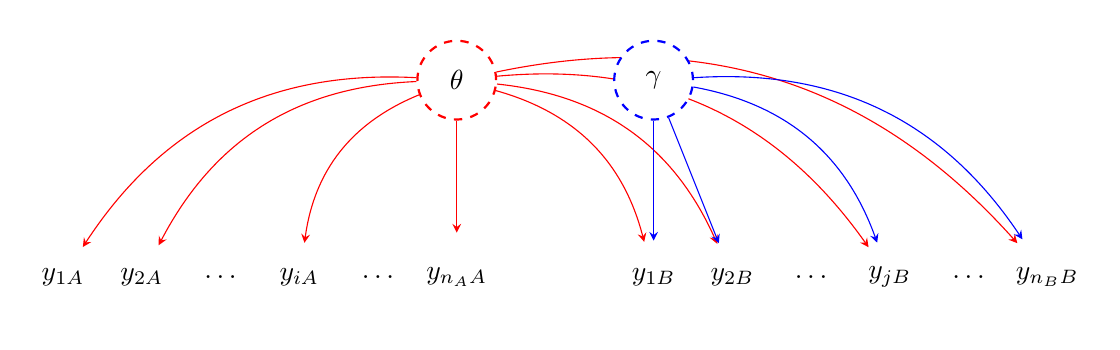
\begin{tikzpicture}[node distance=1cm]
        % styles %
        \tikzstyle{param} = [circle,thick,fill=white,dashed,minimum size=1cm];
        \tikzstyle{yobs} = [circle];
        \tikzstyle{thetadep} = [->, draw=red, fill=red, >=stealth];
        \tikzstyle{gammadep} = [->, draw=blue, fill=blue, >=stealth];
        
        % nodes %
        \node [param,draw=red] (theta) {$\theta$};
        \node [param,draw=blue] (gamma) [right of = theta, xshift = 1.5cm] {$\gamma$};
        
        \node [yobs] (ynA) [below of = theta, yshift=-1.5cm] {$ y_{n_AA} $};
        \node [yobs] (dt1) [left of = ynA] {$ \ldots $};
        \node [yobs] (yiA) [left of = dt1] {$ y_{iA} $};
        \node [yobs] (dt2) [left of = yiA] {$ \ldots $};
        \node [yobs] (y2A) [left of = dt2] {$ y_{2A} $};
        \node [yobs] (y1A) [left of = y2A] {$ y_{1A} $};
        
        \node [yobs] (y1B) [below of = gamma, yshift=-1.5cm] {$ y_{1B} $};
        \node [yobs] (y2B) [right of = y1B] {$ y_{2B} $};
        \node [yobs] (dt3) [right of = y2B] {$ \ldots $};
        \node [yobs] (yjB) [right of = dt3] {$ y_{jB} $};
        \node [yobs] (dt4) [right of = yjB] {$ \ldots $};
        \node [yobs] (ynB) [right of = dt4] {$ y_{n_BB} $};
        
        % edges %
        \begin{pgfonlayer}{background}
        \path[thetadep] (theta) 
                      edge node {} (ynA)
                      edge [bend right] node {} (yiA)
                      edge [bend right] node {} (y2A)
                      edge [bend right] node {} (y1A)
                      edge [bend left]  node {} (y1B)
                      edge [bend left]  node {} (y2B)
                      edge [bend left]  node {} (yjB)
                      edge [bend left]  node {} (ynB);
        \path[gammadep] (gamma)
                      edge node {} (y1B)
                      edge node {} (y2B)
                      edge [bend left] node {} (yjB)
                      edge [bend left] node {} (ynB);
        \end{pgfonlayer}
       \end{tikzpicture}
      \end{figure}
      
      \textbf{Full conditional of $\theta$} \quad The \textit{Markov blanket} of
      $\theta$ is 
      \[ \blanket(\theta) = \left\{ Y_{1A}, Y_{2A}, 
        \ldots, Y_{n_AA}, Y_{1B}, \ldots, Y_{n_BB}, \gamma \right\} \]
      in fact the $\theta$ node does not have parents and its children are all
      the observations. Moreover, for the $ B $ sample, $\gamma$ is another
      parent.
      \begin{align*}
       p(\theta\, |\, \blanket(\theta))
        &\propto p(\theta | a_\theta, b_\theta)\, \prod_{i = 1}^{n_A} p(Y_{iA} | \theta) 
         \prod_{j = 1}^{n_B} p(Y_{jB} | \theta, \gamma) \\
        &= \frac{b_\theta ^ {a_\theta}}{\Gamma(a_\theta)} \theta ^ {a_\theta - 1} \exp(-b_\theta \theta)
         \prod_{i = 1}^{n_A} \theta^{y_{iA}} \frac{\exp(-\theta)}{y_{iA}!}
         \prod_{j = 1}^{n_B} (\theta \cdot \gamma)^{y_{jB}} \frac{\exp(-\theta \gamma)}{y_{jB}!} \\
        &\propto \theta ^ {a_\theta - 1} \exp(-b_\theta \theta)
         \theta ^ {\sum_i y_{iA}} \exp(-n_A \theta) 
         (\theta \cdot \gamma) ^ {\sum_j y_{jB}} \exp(-n_B \theta) \\
        &= \theta ^ {a_\theta + \sum_i y_{iA} + \sum_j y_{jB} - 1} \exp(-(b_\theta + n_A + n_B)\theta)
      \end{align*}
      We can note the kernel of a Gamma distribution, so
      \[ \theta\, |\, \blanket(\theta) \sim \text{Gamma}(a_\theta + 
       \textstyle \sum_i y_{iA} + \textstyle \sum_j y_{jB},\, b_\theta + n_A + n_B) \]
\item \textbf{Full conditional of $\gamma$} \quad The \textit{Markov blanket} of 
      this random variable is
      \[ \blanket(\gamma) = \left\{ Y_{1B}, Y_{2B}, \ldots, Y_{n_BB}, \theta \right\} \]
      \begin{align*}
       p(\gamma\, |\, \blanket(\gamma))
        &\propto p(\gamma | a_\gamma, b_\gamma) \prod_{j = 1}^{n_B} p(y_{jB} | \theta, \gamma) \\
        &= \frac{b_\gamma ^ {a_\gamma}}{\Gamma(a_\gamma)} \gamma^{a_\gamma - 1} \exp(-b_\gamma \gamma)
         \prod_{j = 1}^{n_B} (\theta \cdot \gamma) ^ {y_{iB}} \frac{\exp(-\theta \gamma)}{y_{jB}!} \\
        &\propto \gamma ^ {a_\gamma - 1} \exp(-b_\gamma \gamma) 
         (\theta \cdot \gamma) ^ {\sum_j y_{jB}} \exp(-n_B (\theta \cdot \gamma)) \\
        &\propto \gamma ^ {a_\gamma + \sum_j y_{jB} - 1} \exp(-(b_\gamma + n_B\theta)\gamma)
      \end{align*}
      We can note the kernel of a Gamma distribution, so
      \[ \gamma\, |\, \blanket(\gamma) \sim \text{Gamma}(a_\gamma + \textstyle \sum_j y_{jB},\, 
       b_\gamma + n_B\theta) \]
\item At this point we can proceed with a simulation through the Gibbs algorithm following the MCMC
      approach.
\begin{minted}[fontsize=\small]{r}
library(tidyverse)

# Load data
yobs <- list(
    A = scan("data/menchild30bach.dat"),
    B = scan("data/menchild30nobach.dat")
)

# Hyperparameters
a_theta <- 2
b_theta <- 1
gammapriors <- 2 ^ (3:7)

# Sample statistics
ytot <- map(yobs, sum)
n <- map(yobs, length)

# Simulation main function
library(compiler) # to accelerate
gibbs_sim <- function(a_gamma, b_gamma = a_gamma, 
                      theta0 = 1, gamma0 = 1, nsim = 5000, seed = 10) {
    set.seed(seed)
    # Initialize
    result <- matrix(NA, nsim, 2, dimnames = list(NULL, c("theta", "gamma")))
    result[1, ] <- c(theta0, gamma0)
    # Main loop
    for (r in 2:nsim) {
        result[r, "theta"] <- rgamma(1, a_theta + ytot$A + ytot$B, 
                                     b_theta + n$A + n$B * result[r - 1, "gamma"])
        result[r, "gamma"] <- rgamma(1, a_gamma + ytot$B, b_gamma + n$B * result[r, "theta"])
    }
    # Return
    return(as_tibble(result))
}

# Simulation
simulations <- map(gammapriors, gibbs_sim, nsim = 1E4)
statistics <- map_dbl(simulations, ~ with(., mean(theta * gamma - theta)))
# [1] 0.3720311 0.3344181 0.2713526 0.2000735 0.1327382
\end{minted}
      We have evidence of the fact that the two means converge when the parameters
      of the prior distribution get higher. This imply that the difference gets lower
      and that the mean number of children in the two groups tends to be the same when
      we take higher hyper-parameters.
      
      We can see it even graphically comparing the posterior distributions of $ \theta_A $
      and $ \theta_B $ in the 5 configurations:
\begin{figure}[H]
 \centering
 \includegraphics[width=\linewidth]{r-scripts/week-06_hist.pdf}
\end{figure}
Code:
\begin{minted}[fontsize=\small]{R}
opar <- par(mfrow = n2mfrow(6))

for (j in seq_along(gammapriors)) {
    theta <- pluck(simulations, j, "theta")
    gamma <- pluck(simulations, j, "gamma")
    hist(theta, prob = TRUE, col = "lightblue", ylim = c(0, 5), xlim = c(0, 2.5),
         ylab = "posterior density", xlab = "mean number of children",
         main = substitute(paste(a[gamma], " = ", b[gamma], " = " , prior),
    list(prior = gammapriors[j])))
    lines(density(theta), col = "blue")
    hist(gamma * theta, prob = TRUE, col = "orange", add = TRUE)
    lines(density(gamma * theta), col = "red")
    legend("topleft", c(expression(theta[A]), expression(theta[B])),
           col = c("blue", "red"), lty = 1, cex = 0.7)
}

par(opar)
\end{minted}
      It's apparent even graphically that when the hyper-parameters of $\gamma$ increase, the
      posterior distributions get nearer, going even to overlap.
      
      This is due to the fact that the higher we sat the priors of $\gamma$, the more we
      weight the information that we already have about the variable, and consequently
      the observed information gain less importance.
      
      It's interesting even to observe how the Gamma distribution change when we set the
      different $ a_\gamma $ and $ b_\gamma $.
\begin{figure}[H]
 \centering
 \includegraphics[width=0.65\linewidth]{r-scripts/week-06_prior.pdf}
\end{figure}
      Code:
\begin{minted}[fontsize=\small]{r}
plot(NULL, xlim = c(0, 3), ylim = c(0, 4.5),
     xlab = expression(gamma), ylab = expression(p(gamma)),
     main = "Gamma prior")
for (i in seq_along(gammapriors)) {
    curve(dgamma(x, gammapriors[i], gammapriors[i]), add = TRUE, col = i)
}
legend_txt <- parse(text = paste("a[gamma] ==", gammapriors))
legend(x = 1.5, y = 3, legend_txt, col = seq_along(gammapriors), lty = 1)
mtext(expression(b[gamma] == a[gamma]))
\end{minted}
      As we can see the in the plot, the higher the hyper parameters we set, the
      more the distribution shrinks to 1, that is also the expected value of the
      Gamma. Vice versa, the variance decreases proportionally.
      
      Going toward the limit case in which $ a_\gamma $ and $ b_\gamma $ go to
      infinity we are implicitly affirming that we do not want to \textit{learn}
      anything from the new observations, and we already have a strong opinion
      about the Gamma that we don't want to change. However, if are talking from
      a Bayesian perspective, this situation is not sane neither useful; it's
      just a way to see how much the inference can change on the base of the
      choice of a priori distribution of parameters.
      
      \textbf{Observation} \quad It would be appropriate to adequately assess
      the convergence of the Gibbs algorithm, but in this case it was not done
      because it was not explicitly requested by the exercise. We just calculate
      the effective sample size and make sure it is high enough to make sure we
      have reached the equilibrium distribution and have it very close to it.
      
\begin{minted}[fontsize=\small]{r}
library(coda)
map(simulations, effectiveSize)

# [[1]]
# theta    gamma
# 1175.254 1198.183
#
# [[2]]
# theta    gamma
# 1471.870 1353.061
#
# [[3]]
# theta    gamma
# 1840.738 1695.119
#
# [[4]]
# theta    gamma
# 2424.931 2238.538
#
# [[5]]
# theta    gamma
# 3259.088 2942.661
\end{minted}
\end{enumerate}

\part{}
\chapter{Hierarchical models, part 1}

\section{Exercise 8.1, Hoff}

\subsection{Data}
\begin{itemize}
 \item Consider the hierarchical model where
       \begin{align*}
        \theta_1, \ldots, \theta_m   | \mu, \tau^2        & \sim \iid \Normal(\mu,
        \tau^2)
        \\
        y_{1, j}, \ldots, y_{n_j, j} | \theta_j, \sigma^2 & \sim \iid \Normal(\theta_j,
        \sigma^2)
       \end{align*}
\end{itemize}

\subsection{Questions}
\begin{enumerate}[label=\alph*)]
 \item Which do you think is bigger, $ \Var[y_{i, j} | \theta_i, \sigma^2] $ or $
        \Var[y_{i, j} | \mu, \tau^2] $?
 \item Do you think $ \Cov[y_{i_1, j}, y_{i_2, j} | \theta_j, \sigma^2] $ is negative,
       positive or zero?
       Answer the same for $ \Cov[y_{i_1, j}, y_{i_2, j} | \mu, \tau^2] $.
 \item Compute the quantities and compare with the intuitive results.
 \item Assuming that we had a prior $ p(\mu) $ for $\mu$. Using the Bayes' rule, show
       that
       \[ p(\mu | \theta_1, \ldots, \theta_m, \tau^2, \sigma^2, \vect y_1, \ldots, \vect
        y_m) =
        p(\mu | \theta_1, \ldots, \theta_m, \tau^2) \]
       Interpret in words what this means.
\end{enumerate}

\subsection{Solutions}
\begin{enumerate}[label=\alph*)]
 \item $ \Var[y_{i, j} | \mu, \tau^2] $ will be intuitively the higher one, because we
       are \textit{constraining}
       fewer variables.
 \item The two variables $ y_{i_1, j} $ and $ y_{i_2, j} $ will be independent given $
        \theta_j $, for definition.
       Yet, if I condition only on $ \mu $ and $ \tau^2 $, the two variables will have a
       positive covariance; in fact
       if I observe a high value of $ y_{i_1, j} $ I expect to see a similar value for $
        y_{i_2, j} $ and vice versa.
 \item \begin{align*}
        \intertext{\raggedleft By definition, we know that $ y_{i, j} | \theta_j,
          \sigma^2
          \sim \Normal(\theta_j, \sigma^2) $}
        \Var[y_{i, j} | \theta_j, \sigma^2]
         & = \sigma^2
        \\
        \intertext{\raggedleft We can apply the property of variance of independent
         variables,
         \\
         because $ y_{i, j} | \theta_j, \sigma^2 $ are i.i.d.}
        \Var[\bar y_j | \theta_j, \sigma^2]
         & = \Var\left[ \frac{1}{n} \sum_{i = 1}^{n} y_{i, j} | \theta_j, \sigma^2
         \right]
        \\
         & = \frac{1}{n} \sum_{i = 1}^{n} \Var[y_{i, j} | \theta_j, \sigma^2] =
        \frac{\sigma^2}{n_j}
        \\
        \intertext{\raggedleft Again using the property that $ y_{i, j} $ are i.i.d.,
         given
         $ \theta_j $ and $ \sigma^2 $}
        \Cov[y_{i_1, j}, y_{i_2, j} | \theta_j, \sigma^2]
         & = 0
        \\
        \intertext{\centering The first intuition of point b) was correct, and justified
         by theory.}
       \end{align*}

       \setlength{\fboxsep}{10pt} % increase the spacing of fbox
       \fbox{\parbox{\textwidth}{ % put everything inside a frame
         \textbf{Note} \quad This quantities concern variables conditioned to a generic
         group \textit{j},
         and it is straightforward to obtain them even in a frequentist point of view.
         The next variances require to consider these theorems of probability theory:
         \begin{enumerate}
          \item \textbf{Law of total variance}: \\
                Given two random variables $ X $ and $ Y $ with $ \Var[X] < \infty $,
                then:
                \begin{equation}\label{week7:eq_totalvariance}
                 \Var[X] = \E[\Var[X | Y]] + \Var[\E[X | Y]]
                \end{equation}
          \item \textbf{Law of total covariance}: \\
                Given three random variables $ X $, $ Y $ and $ Z $ with $ \Cov[X, Y] <
                 \infty $, then:
                \begin{equation}\label{week7:eq_totalcovariance}
                 \Cov[X, Y | Z] = \E[\Cov[X, Y | Z]] + \Cov[\E[X | Z] \cdot \E[Y | Z]]
                \end{equation}
         \end{enumerate}
        }}

       \begin{align*}
        \intertext{\raggedleft Thus, we can apply here \ref{week7:eq_totalvariance} with
         $ X = y_{i, j} $ and $ Y = \theta_j $}
        \Var[y_{i, j} | \mu, \tau^2]
         & = \E[\Var[y_{i, j} | \theta_j, \mu, \tau^2]] + \Var[\E[y_{i, j} | \theta_j,
          \mu,
          \tau^2]]
        \\
         & = \E[\Var[y_{i, j} | \theta_j, \sigma^2, \mu, \tau^2]] +
        \Var[\E[y_{i, j} | \theta_j, \sigma^2, \mu, \tau^2]]
        \\
         & = \E[\sigma^2] + \Var[\theta_j | \mu, \tau^2]
        \\
         & = \sigma^2 + \tau^2 > \sigma^2
        \\
        \intertext{\centering The intuition at point a) is confirmed.}
        \intertext{\raggedleft We apply again \ref{week7:eq_totalvariance}, with $ X =
          \bar y_j $ and $ Y = \theta_j $}
        \Var[\bar y_j | \mu, \tau^2]
         & = \E[\Var[\bar y_j | \theta_j, \mu, \tau^2]] + \Var[\E[\bar y_j | \theta_j,
          \mu,
          \tau^2]]
        \\
         & = \E[\Var[\bar y_j | \theta_j, \sigma^2, \mu, \tau^2]] +
        \Var[\E[\bar y_j | \theta_j, \sigma^2, \mu, \tau^2]]
        \\
         & = \E[\frac{\sigma^2}{n_j}] + \Var[\theta_j | \mu, \tau^2] =
        \frac{\sigma^2}{n_j}
        + \tau^2
        \\
        \intertext{\raggedleft Lastly, we use \ref{week7:eq_totalcovariance} for the last
         term with
         $ X = y_{i_1, j} $, $ Y = y_{i_2, j} $ and $ Z = \theta_j $}
        \Cov[y_{i_1, j}, y_{i_2, j} | \mu, \tau^2]
         & = \E[\Cov[y_{i_1, j}, y_{i_2, j} | \theta_j, \mu, \tau^2]]
        \\
         & + \Cov[\E[y_{i_1, j} | \theta_j, \mu, \tau^2] \cdot \E[y_{i_2, j} | \theta_j,
          \mu, \tau]]
        \\
         & = \E[0] + \Cov[\theta_j, \theta_j | \mu, \tau^2]
        \\
         & = 0 + \Var[\theta_j | \mu, \tau^2] = \tau^2 > 0
        \intertext{\centering Even the second intuition of the point b) was correct.}
       \end{align*}
       \textbf{Note} \quad Another analytic solution could be to calculate the marginal
       distribution of $ y_{i, j} | \mu, \tau^2 $ as
       \[ p(y_{i, j} | \theta_j, \mu, \tau^2) =
        \int_{\theta_j \in \Theta} p(y_{i, j} | \theta_j, \mu, \tau^2) \cdot p(\theta_j |
        \mu, \tau^2) \partial \theta_j \]
       Since both of them are normal distributions, we expect it to be another normal,
       and we have only to verify that
       the variance is equal to $ \Var[y_{i, j} | \mu, \tau^2] $ as previously computed.
       The same for the other quantities.
 \item First of all, we represent the hierarchical model through a DAG
       \begin{figure}[H]
        \centering
        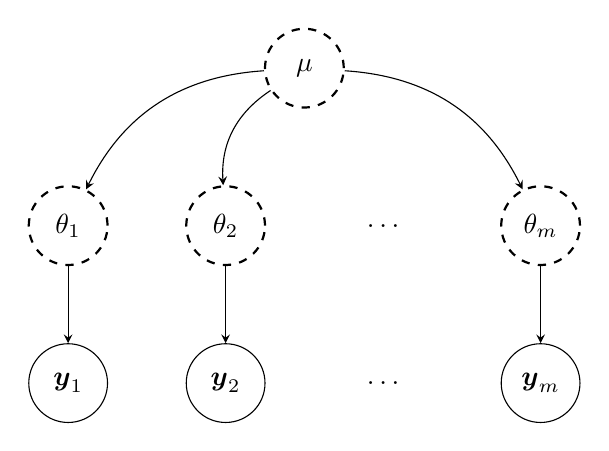
\begin{tikzpicture}[node distance=1cm,->,draw=black,>=stealth]
         % styles %
         \tikzstyle{param} = [circle,thick,draw=black,fill=white,dashed,minimum
         size=1cm];
         \tikzstyle{yobs} = [circle,draw=black,fill=white,minimum size=1cm];

         % nodes %
         \node [param] (mu) {$\mu$};

         \node [param,below of=mu, yshift=-1cm, xshift=-1cm] (theta2) {$\theta_2$};
         \node [param,draw=white,below of=mu, yshift=-1cm, xshift=1cm] (thetadots)
         {$\ldots$};
         \node [param,left of=theta2, xshift=-1cm] (theta1) {$\theta_1$};
         \node [param,right of=thetadots, xshift=1cm] (thetam) {$\theta_m$};

         \node [yobs,below of=theta1,yshift=-1cm] (y1) {$\vect y_1$};
         \node [yobs,below of=theta2,yshift=-1cm] (y2) {$\vect y_2$};
         \node [yobs,draw=white,below of=thetadots,yshift=-1cm] (ydots) {$\ldots$};
         \node [yobs,below of=thetam,yshift=-1cm] (ym) {$\vect y_m$};

         % edges %

         \path (mu)
         edge [bend right] node {} (theta1)
         edge [bend right] node {} (theta2)
         edge [bend left] node {} (thetam);
         \path (theta1) edge node {} (y1);
         \path (theta2) edge node {} (y2);
         \path (thetam) edge node {} (ym);
        \end{tikzpicture}
       \end{figure}
       Using this graph and its factorization one can calculate the conditioned
       probability as
       \begin{align*}
        p(\mu | \theta_1, \ldots, \theta_m, \tau^2, \sigma^2, \vect y_1, \ldots, \vect
        y_m)
         & = \frac{p(\mu, \theta_1, \ldots, \theta_m, \tau^2, \sigma^2, \vect y_1,
         \ldots,
         \vect y_m)}
        {p(\theta_1, \ldots, \theta_m, \tau^2, \sigma^2, \vect y_1, \ldots,
         \vect y_m)}
        \\
         & = \frac{p(\mu, \theta_1, \ldots, \theta_m, \tau^2, \sigma^2, \vect y_1,
         \ldots,
         \vect y_m)}
        {\int p(\mu, \theta_1, \ldots, \theta_m, \tau^2, \sigma^2, \vect y_1,
         \ldots, \vect y_m) \dd \mu}
        \\
         & = \frac{p(\vect y_1, \ldots, \vect y_m | \theta_1, \ldots, \theta_m, \sigma^2)
         \cdot
         p(\theta_1, \ldots, \theta_m | \mu, \tau^2) \cdot p(\mu)}
        {\int p(\vect y_1, \ldots, \vect y_m | \theta_1, \ldots, \theta_m,
         \sigma^2) \cdot
         p(\theta_1, \ldots, \theta_m | \mu, \tau^2) \cdot p(\mu) \dd \mu}
        \\
         & = \frac{p(\vect y_1, \ldots, \vect y_m | \theta_1, \ldots, \theta_m, \sigma^2)
         \cdot
         p(\theta_1, \ldots, \theta_m | \mu, \tau^2) \cdot p(\mu)}
        {p(\vect y_1, \ldots, \vect y_m | \theta_1, \ldots, \theta_m, \sigma^2)
         \cdot
         \int p(\theta_1, \ldots, \theta_m | \mu, \tau^2) \cdot p(\mu) \dd \mu}
        \\
         & = \frac{p(\theta_1, \ldots, \theta_m | \mu, \tau^2) \cdot p(\mu)}
        {\int p(\theta_1, \ldots, \theta_m | \mu, \tau^2) \cdot p(\mu) \dd \mu}
        \\
         & = \frac{p(\theta_1, \ldots, \theta_m, \mu, \tau^2)}{p(\theta_1, \ldots,
         \theta_m, \tau^2)}
        \\
         & = p(\mu | \theta_1, \ldots, \theta_m, \tau^2) \tag*{$ \square $}
       \end{align*}

       This result implies that the information obtained from the samples in a
       certain sense does not refer \textit{directly} on the grand mean, but it
       passes trough the inference that we do on $\theta$s. In fact, the grand mean
       is independent of the observations conditioned $ \theta_1, \ldots, \theta_m $.
\end{enumerate}

\section{Exercise on continuous mixture models}

\subsection{Data}
\begin{itemize}
 \item If $ y|\theta \sim \Poisson(\theta) $ and $ \theta \sim \Gammadist(\alpha,
       \beta) $, then the marginal (prior predictive) distribution of $ y $ is a
       negative binomial with parameters $\alpha$ and $\beta$ (or $ p = \beta / (1 +
       \beta) $).
 \item In the Normal model with unknown location and scale ($\mu$, $\sigma^2$),
       the non informative prior density, $ p(\mu, \sigma) \propto 1 / \sigma^2 $,
       results in a normal-inverse-$\chi^2$ posterior distribution. Marginally then
       $ \sqrt{n} (\mu - \bar y) / s $ has a posterior distribution $ t_{n - 1} $,
       where $ s^2 = \sum_i (y_i - \bar y)^2 / (n - 1) $ is the sample
       variance of the observation.
\end{itemize}

\subsection{Questions}
\begin{enumerate}[label=\alph*)]
 \item Derive the mean and the variance of the negative binomial.
 \item Derive the first two moments of the latter distribution, stating the
       appropriate condition on $n$ for existence of both of them.
\end{enumerate}

\subsection{Solutions}
\begin{enumerate}[label=\alph*)]
 \item We can leverage on the property of the expected value that, given two variables
       $ X $ and $ Y $
       \begin{equation}\label{week7:eq_condexpectation}
        \E_X[X] = \E_Y[\E_X[X | Y]]
       \end{equation}
       Thus,
       \begin{align*}
        \E_y[y] & = \E_\theta[\E_y[y | \theta]] \\
                & = \E_\theta[\theta]           \\
                & = \frac{\alpha}{\beta}
       \end{align*}

       For the variance, we can refer to \ref{week7:eq_totalvariance} and consider
       $ X = y $ and $ Y = \theta $
       \begin{align*}
        \Var[y] & = \E[\Var[y | \theta]] + \Var[\E[y | \theta]]   \\
                & = \E[\theta] + \Var[\theta]                     \\
                & = \frac{\alpha}{\beta} + \frac{\alpha}{\beta^2} \\
                & = \frac{(1 + \beta) \alpha}{\beta^2}
       \end{align*}

       \textbf{Formal alternative} \quad Using the following parameterization:
       \[ p(x | \theta, r) = \binom{x - 1}{r - 1} \theta ^{r} (1 - \theta) ^{x - r} \]
       with $ \theta = \beta / ( 1 + \beta) $ and $ r = \alpha $.

       \begin{align*}
        \E[x] & = \sum_{x \in \Theta} x \cdot p(x)
        \\
              & = \sum_{x = r}^{\infty} x \cdot \binom{x - 1}{r - 1} \cdot \theta ^r (1 -
        \theta) ^{x - r}
        \\
              & = \sum_{x = r}^{\infty} x \cdot \frac{(x - 1)!}{(r - 1)!(x - r)!} \cdot
        \theta ^r (1 - \theta) ^{x - r}
        \\
              & = r \cdot \sum_{x = r}^{\infty} \frac{x!}{r!(x - r)!} \cdot \theta ^r (1
        -
        \theta) ^{x - r}
        \intertext{\raggedleft Increment the lower index of the summation
         \\
         and decrement the index in the summand}
              & = \frac{r}{\theta} \cdot \sum_{x = r + 1}^{\infty} \binom{x - 1}{(r + 1)
         -
         1}
        \theta ^{r + 1} (1 - \theta) ^{x - (r + 1)}
        \intertext{\raggedleft The series is the sum of the PDF function of a $
          \text{NegBin}(\theta, r + 1) $
         \\
         all along its support, thus it is equal to 1}
              & = \frac{r}{\theta}
       \end{align*}

       To obtain the variance we recur to the equality
       \begin{equation}\label{week7:eq_variance}
        \Var[X] = \E[X^2] - \E[X]^2
       \end{equation}
       so, we obtain first of all $ \E[X^2] $.
       \begin{align*}
        \E[X^2]          & = \sum_{x = r}^{\infty} x^2 \cdot \binom{x - 1}{r - 1} \cdot
        \theta ^r
        (1 - \theta) ^{x - r}
        \\
                         & = \sum_{x = r}^{\infty} [x(x + 1) - x] \binom{x - 1}{r - 1}
        \cdot \theta
        ^r (1 - \theta) ^{x - r}
        \\
                         & = \sum_{x = r}^{\infty} [x(x + 1)] \binom{x - 1}{r - 1} \cdot
        \theta ^r
        (1 - \theta) ^{x - r} -
        \sum_{x = r}^{\infty} x \cdot \binom{x - 1}{r - 1} \cdot \theta ^r (1 -
        \theta) ^{x - r}
        \\
        \intertext{\raggedleft Following the same reasoning of the mean
         expression:
         \\
         multiply and divide for $ r $ and then $ r + 1 $}
                         & = \frac{r(r + 1)}{\theta ^2} \sum_{x = r + 2} \binom{x + 1}{r
         + 1} \theta
        ^{x + 2} (1 - \theta) ^{x - (r + 2)} -
        \frac{r}{\theta}
        \\
                         & = \frac{r(r + 1)}{\theta ^2} - \frac{r}{\theta}
        \\
                         & = \frac{r^2 + r - \theta r}{\theta ^2}
        \\
                         & = \frac{r^2}{\theta^2} + \frac{(1 - \theta) r}{\theta^2}
        \\
        \intertext{\raggedleft Now we can apply \ref{week7:eq_variance}}
        \implies \Var[X] & = \frac{r^2}{\theta^2} + \frac{(1 - \theta) r}{\theta^2} -
        \left( \frac{r}{\theta} \right)^2
        \\
                         & = \frac{(1 - \theta)r}{\theta ^ 2}
       \end{align*}
 \item The PDF of Student's t distribution
       \[ p(x | n) = c \cdot \left( 1 + \frac{x^2}{n} \right)^{-\frac{n + 1}{2}} \]
       where the c is a constant
       \[ c = \frac{1}{\sqrt{n}} \frac{1}{\Beta\left( \frac{n}{2}, \frac{1}{2}
       \right)} \]
       and $ \Beta(\parm, \parm) $ is the Beta function.

       It's immediate to see that the function is even, because $ x $ is present
       only as $ x^2 $, hence $ f(-x) = f(x) $.
       \begin{align*}
        \E[X] & = \int_{x \in \Theta} x \cdot f(x)  \dd x                         \\
              & = \int_{-\infty}^{\infty} x \cdot f(x) \dd x                      \\
              & = \int_{-\infty}^{0} x \cdot f(x) \dd x +
        \int_{0}^{\infty} x \cdot f(x) \dd x                                      \\
        \intertext{\raggedleft Change of variable in the first
         integral                                                                 \\$ t =
         -x $}
              & = -\int_{\infty}^{0} (-t) \cdot f(-t) \dd t +
        \int_{0}^{\infty} x \cdot f(x) \dd x                                      \\
              & = \phantom{-} \int_{\infty}^{0} \phantom{-} t \cdot f(-t) \dd t +
        \int_{0}^{\infty} x \cdot f(x) \dd x                                      \\
              & = -\int_{0}^{\infty} t \cdot f(-t) \dd t +
        \int_{0}^{\infty} x \cdot f(x) \dd x                                      \\
        \intertext{\raggedleft Since $ f(x) = f(-x) $}
              & = -\int_{0}^{\infty} t \cdot f(t) \dd t + \int_{0}^{\infty} x
        \cdot f(x) \dd x = 0
       \end{align*}
       The equality to 0 is granted by the finiteness of the two integrals, that
       is true only if the parameter $ n $ of the distribution is strictly
       greater then 1. In fact
       \begin{align*}
        \int_{0}^{\infty} x f(x) \dd x
         & = \lim\limits_{u \to \infty} \int_{0}^{u} x \cdot c \cdot
        \left( 1 + \frac{x^2}{n} \right)^{-\frac{1}{2}(n + 1)} \dd x    \\
         & = c \cdot \lim\limits_{u \to \infty} \left.
        -\frac{n}{n - 1} \left( 1 + \frac{x^2}{n} \right)^{-\frac{1}{2}(n - 1)}
        \right| _{0} ^{u}                                               \\
         & = -\frac{c \cdot n}{n - 1} \left( \lim\limits_{u \to \infty}
        \left( 1 + \frac{u^2}{n} \right)^{-\frac{1}{2}(n - 1)} - 1 \right)
       \end{align*}
       And the above limit is finite only if $ n > 1 $.

       \begin{align*}
        \E[X^2]
         & = \int_{x \in \Theta} x^2 \cdot f(x) \dd x
        \\
         & = \int_{-\infty}^{\infty} x^2 \cdot c \cdot \left( 1 + \frac{x^2}{n}
        \right)^{-\frac{n + 1}{2}} \dd x
        \intertext{\raggedleft Change of variable $ t = \left( 1 + \frac{x^2}{n}
          \right)^{-1} $}
         & = n ^{\frac{3}{2}} \cdot c \cdot \int_{0}^{1} t ^{\frac{n}{2} - 2} (1 - t)
        ^{\frac{1}{2}} \dd t
        \\
        \intertext{\raggedleft Note that the integrand function is the kernel of a Beta
         distribution,
         \\
         thus its result is known.}
         & = n ^{\frac{3}{2}} \cdot c \cdot \Beta\left( \frac{n}{2} - 1, \frac{3}{2}
        \right)
        \\
         & = n ^{\frac{3}{2}} \cdot \frac{1}{\sqrt{n} \Beta\left( \frac{n}{2},
         \frac{1}{2}
         \right)} \cdot
        \Beta\left( \frac{n}{2} - 1, \frac{3}{2} \right)
        \\
         & = n \cdot \frac{\Gamma\left( \frac{n}{2} + \frac{1}{2} \right)}
        {\Gamma\left( \frac{n}{2} \right) \Gamma\left( \frac{1}{2}
         \right)}
        \frac{\Gamma\left( \frac{n}{2} - 1 \right) \Gamma\left( \frac{3}{2}
         \right)}
        {\Gamma\left( \frac{n}{2} + \frac{1}{2} \right)}
        \\
        \intertext{\raggedleft By the property of the Gamma function that
         \\
         $ \Gamma(x) = (x - 1) \Gamma(x - 1) $}
         & = n \cdot \frac{\Gamma\left( \frac{n}{2} - 1 \right) \frac{1}{2} \Gamma\left(
         \frac{1}{2} \right)}
        {\left(\frac{n}{2} - 1\right) \Gamma\left( \frac{n}{2} - 1
         \right) \Gamma\left( \frac{1}{2} \right)}
        \\
         & = \frac{n}{n - 2}
       \end{align*}
       In this case the condition is $ n > 2 $, otherwise the integral of the
       Beta distribution does not converge.
\end{enumerate}

\chapter{Hierarchical models, part 2}

\section{Exercise 1}

\subsection{Questions}
Demonstrate that $ \text{SSR}_g $ (defined like at page 158 of Hoff's book)
converge to
\[ \text{SSR}_{\text{OLS}} = \sum (y_i	- \vect{\hat \beta}_\text{OLS} \vect x_i)^2 \]
when $ g \to \infty $.

\subsection{Solutions}
\[ \text{SSR}_g = \vect y' \vect y - \vect m' \vect V ^{-1} \vect y =
 \vect y' \left( I - \frac{g}{g + 1} X (X'X)^{-1} X' \right) \vect y \]
By definition $ \text{SSR}_\text{OLS} $ can be written as
\begin{align*}
 \text{SSR}_\text{OLS} & = \sum (y_i  - \vect{\hat \beta}_\text{OLS} \vect x_i)^2 \\
                       & = \vect y' \left( I - X(X'X)^{-1}X' \right) \vect y
\end{align*}
So, it is apparent that when I take the limit
\[ \lim\limits_{g \to \infty} \text{SSR}_g = \text{SSR}_\text{OLS} \]
Because the value $ \frac{g}{g + 1} $ converges to 1.

\section{Exercise 9.2, Hoff}

\subsection{Data}
Model selection: As described in Example 6 of Chapter 7, The file
\texttt{azdiabetes.dat} contains data on health-related variables of a
population of 532 women. In this exercise we will be modeling the conditional
distribution of glucose level (\texttt{glu}) as a linear combination of the
other variables, excluding the variable diabetes.

\subsection{Questions}
\begin{enumerate}[label=\alph*) ]
 \item Fit a regression model using a \textit{g}-prior with $ g = n $,
       $ \nu_0 = 2 $ and $ \sigma^2_0 = 1 $. Obtain a posterior confidence
       intervals for all the parameters.
 \item Perform a model selection and averaging procedure described in
       Section 9.3. Obtain $ \Pr(\beta_j \ne 0 | \vect y) $, as well as
       posterior confidence intervals for all the parameters. Compare
       to the results in part a).
\end{enumerate}

\subsection{Solutions}
\begin{enumerate}[label=\alph*) ]
 \item \textbf{Code}
       \begin{minted}{R}
library(tidyverse)
library(compiler)
set.seed(1)

# loading data
dataset <- read_csv("data/azdiabetes.dat", col_names = TRUE)
N <- nrow(dataset)

y <- dataset$glu
X <- model.matrix(glu ~ ., data = dataset)

# rescale when numeric: (y - mean) / sd
y <- scale(y)
X <- apply(X, 2, function(x) if (length(unique(x)) > 2) scale(x) else x)

# OLS modeling
lsfit <- lm(y ~ X - 1)

# G prior
Id <- function(n) diag(1, n)

lmgprior <- function(y, X, g = NROW(X),
                nu_0 = 1, s2_0 = try(summary(lm(y ~ X - 1))$sigma ^ 2, silent = TRUE),
                S = 5000) {
   n <- NROW(X)
   p <- NCOL(X)

   H_g   <- (g / (g + 1)) * X %*% solve(t(X) %*% X) %*% t(X)
   SSR_g <- c(t(y) %*% (Id(n) - H_g) %*% y)
   s2    <- 1 / rgamma(S, (nu_0 + n) / 2, (nu_0 * s2_0 + SSR_g) / 2)

   V_b <- g * solve(t(X) %*% X) / (g + 1)
   E_b <- V_b %*% t(X) %*% y # Expected value of the posterior

   # Use the s2 sampled from the inv-gamma
   E <- matrix(rnorm(S * p, 0, sqrt(s2)), S, p)

   # Sampling from a normal centered in E_b and with variance s2 * V_b
   # beta = E_b + E * chol(V_b), E ~ N(0, s2 * I)
   beta <- t(t(E %*% chol(V_b)) + c(E_b))

   # Return
   list(beta = beta, s2 = s2)
}

lmgpriorfit <- lmgprior(y, X, g = N, nu_0 = 2, s2_0 = 1)

beta_gprior <- apply(lmgpriorfit$beta, 2,
                     function(x) quantile(x, c(0.025, 0.975)))
\end{minted}

       \textbf{Coefficients}
       % latex table generated in R 3.5.1 by xtable 1.8-3 package
       % Sun Nov 25 15:39:43 2018
       \begin{table}[ht]
        \centering
        \begin{tabular}{rrrrrrrrr}
         \hline
                & (Intercept) & npreg & bp    & skin  & bmi   & ped   & age  &
         diabetesYes
         \\
         \hline
         2.5\%  & -0.39       & -0.21 & -0.00 & -0.05 & -0.05 & -0.04 & 0.08 & 0.74
         \\
         97.5\% & -0.21       & -0.02 & 0.16  & 0.15  & 0.15  & 0.11  & 0.28 & 1.07
         \\
         \hline
        \end{tabular}
       \end{table}

 \item \textbf{Code}
       \begin{minted}{R}
set.seed(1)

backselect_tcrit <- function(y, X, tcrit = qnorm(0.975)) {
   Xc <- X
   remaining <- 1:NCOL(X)

   repeat {
      if (!is_empty(remaining)) {
         fit   <- lm(y ~ Xc - 1)
         summ  <- summary(fit)
         tstat <- summ$coef[, 3]
         s2    <- summ$sigma ^ 2
      } else break
      jpmax <- which.min(abs(tstat))
      Xc <- Xc[, -jpmax, drop = FALSE]
      remaining <- remaining[-jpmax]

      if ( (all(abs(tstat) > tcrit) || is_empty(remaining)) ) break
   }

   # Return
   list(remaining = remaining, removed = setdiff(1:NCOL(X), remaining))
}

loglikpy_X <- function(y, X, g = NCOL(X),
                       nu_0 = 1,
                       s2_0 = try(summary(lm(y ~ X - 1))$sigma ^ 2,
                                  silent = TRUE)) {
   n <- NROW(X)
   p <- NCOL(X)

   if (p == 0) s2_0 <- mean(y ^ 2)
   H_0 <- 0
   if (p > 0) H_0 <- g / (g + 1) * X %*% solve(t(X) %*% X) %*% t(X)
   SSR_g <- c(t(y) %*% (Id(n) - H_0) %*% y)

   # Return
   - 0.5 * n * log(2 * pi) + lgamma(0.5 * (nu_0 + n)) - lgamma(0.5 + nu_0) +
      - 0.5 * p * log(1 + g) + 0.5 * nu_0 * log(0.5 * nu_0 * s2_0) +
      - 0.5 * (nu_0 + n) * log(0.5 * (nu_0 * s2_0 + SSR_g))
}

# model selection (backward elimination)
variables <- backselect_tcrit(y, X, tcrit = 1.65)
Xred <- X[, variables$remaining]
reducedlmfit <- lm(y ~ Xred - 1)

# model averaging
p <- NCOL(X)
S <- 500
B <- matrix(NA, S, p, dimnames = list(NULL, colnames(X)))
Z <- matrix(NA, S, p, dimnames = list(NULL, colnames(X)))
z <- rep(TRUE, p)

lpy_0 <- loglikpy_X(y, X[, z])

for (iter in 1:S) {
   for (j in sample(1:p)) {
      zp    <- z # include/exclude a sampled regressor
      zp[j] <- !zp[j]
      lpy_p <- loglikpy_X(y, X[, zp])
      r     <- (lpy_p - lpy_0) * (-1) ^ (!zp[j])

      # Note: Prior on z gives same prior probability to all models
      z[j] <- rbinom(1, 1, 1 / (1 + exp(-r))) == 1
      if (z[j] == zp[j]) lpy_0 <- lpy_p
   }

   beta <- z
   if (sum(z) > 0) {
      beta[z] <- lmgprior(y, X[, z, drop = FALSE], S = 1) %>%
         purrr::pluck("beta")
   }

   Z[iter, ] <- z
   B[iter, ] <- beta
}

beta_bma <- apply(B, 2, quantile, c(0.025, 0.975), na.rm = TRUE)
prob_include <- apply(Z, 2, mean)
\end{minted}

       \textbf{Coefficients}
       % latex table generated in R 3.5.1 by xtable 1.8-3 package
       % Sun Nov 25 15:38:39 2018
       \begin{table}[ht]
        \centering
        \begin{tabular}{rrrrrrrrr}
         \hline
                & (Intercept) & npreg & bp   & skin  & bmi   & ped   & age  & diabetesYes
         \\
         \hline
         2.5\%  & -0.40       & -0.21 & 0.00 & -0.03 & -0.05 & -0.03 & 0.06 & 0.72
         \\
         97.5\% & -0.22       & 0.00  & 0.16 & 0.14  & 0.14  & 0.12  & 0.28 &
         1.09
         \\
         \hline
        \end{tabular}
       \end{table}

       \textbf{Inclusion probability}
       % latex table generated in R 3.5.1 by xtable 1.8-3 package
       % Sun Nov 25 15:50:44 2018
       \begin{table}[ht]
        \centering
        \begin{tabular}{rrrrrrrrr}
         \hline
         (Intercept) & npreg & bp   & skin & bmi  & ped  & age  & diabetesYes &
         \\
         \hline
         1.00        & 0.95  & 0.86 & 0.72 & 0.70 & 0.72 & 0.99 & 1.00        &
         \\
         \hline
        \end{tabular}
       \end{table}
\end{enumerate}

\chapter{Bayesian GLM}

\section{Exercise 10.1, Hoff}

\subsection{Data}
Reflecting random walks: It is often useful in MCMC to have a proposal
distribution which is both symmetric and has support only on a certain
region. For example, if we know $ \theta > 0 $, we would like our proposal
distribution $ J(\theta_1 | \theta_0) $ to have support on positive $ \theta $
values. Consider the following algorithm:
\begin{enumerate}
 \item sample $ \tilde \theta \sim \Unif(\theta_0 - \delta, \theta_0 + \delta) $;
 \item $ \theta_1 \overset{!}{=} \begin{cases} -\tilde \theta          & \text{if }
         \tilde \theta < 0                                        \\
         \phantom- \tilde \theta & \text{if } \tilde \theta \ge 0 \end{cases} $
\end{enumerate}
In other words $ \theta_1 = | \tilde \theta | $.

\subsection{Questions}
Show that the above algorithm draws samples from a symmetric proposal distribution
which has support on positive values of $ \theta $. It may be helpful to write out
the associated proposal density $ J(\theta_1 | \theta_0) $ under the two conditions
$ \theta_0 < \delta $ and $ \theta_0 \ge \delta $ separately.

\subsection{Solutions}
To demonstrate that the algorithm draws from a symmetric distribution we have to 
show that \[ J(\theta_1 | \theta_0) = J(\theta_0 | \theta_1) \]

\begin{equation*}
 J(\theta_1 | \theta_0) = \begin{cases} 
    \frac{1}{2 \delta} \mathbf{1}_{(\theta_0 - \delta, \theta_0 + \delta]}(\theta_1) & \text{if } \theta_0 \ge \delta 
      \text{ \large \textcircled{\small 1}} \\
    \frac{1}{\delta} \mathbf{1}_{(0, \delta - \theta_0]}(\theta_1) + 
      \frac{1}{2 \delta} \mathbf{1}_{[\delta - \theta_1, \delta + \theta_1]}(\theta_0) & \text{if } \theta_0 < \delta
      \text{ \large \textcircled{\small 2}}
  \end{cases}
\end{equation*}

equivalently

\begin{equation*}
  J(\theta_0 | \theta_1) = \begin{cases}
    \frac{1}{2 \delta} \mathbf{1}_{(\theta_1 - \delta, \theta_1 + \delta]}(\theta_0) & \text{if } \theta_1 \ge \delta 
      \text{ \large \textcircled{\small 1}}\\
    \frac{1}{\delta} \mathbf{1}_{(0, \delta - \theta_1]}(\theta_0) + 
      \frac{1}{2 \delta} \mathbf{1}_{[\delta - \theta_0, \delta + \theta_0]}(\theta_1) & \text{if } \theta_1 < \delta
      \text{ \large \textcircled{\small 2}}
  \end{cases}
\end{equation*}

\subsubsection{Case 1: $ \theta_0 \ge \delta, \theta_1 \ge \delta $}
For both $ J(\theta_1 | \theta_0) $ and $ J(\theta_0 | \theta_1) $ we are in the case
{\large \textcircled{\small 1}}, thus they have same density $ \frac{1}{2 \delta} $.

\subsubsection{Case 2: $ \theta_0 \ge \delta, \theta_1 < \delta $}
$ J(\theta_1 | \theta_0) = \frac{1}{2 \delta} $ (since it falls in case 
{\large \textcircled{\small 1}}), but when does it equals $ J(\theta_0 | \theta_1) $?
Since $ \theta_1 < \delta $ we have to concentrate on the ``bottom'' to have 
$ J(\theta_0 | \theta_1) = \frac{1}{\delta} $ (see case {\large \textcircled{\small 2}}):
\begin{align*}
  \max(\delta - \theta_1) &\le \theta_0 \\
  \delta - \min(\theta_1) &\le \theta_0 \\
  \intertext{\centering but since $ \theta_0 \in [\delta - \theta_1, \delta + \theta_1] $}
  \delta - (\theta_0 - \delta) &\le \theta_0 \\
  2 \delta &\le 2 \theta_0 \\
  \delta &\le \theta_0 \tag*{$ \checkmark $}
\end{align*}

\subsubsection{Case 3: $ \theta_0 < \delta, \theta_1 \ge \delta $}
For $ \theta_1 \ge \delta $ we are in the case {\large \textcircled{\small 1}},
thus $ J(\theta_0 | \theta_1) = \frac{1}{2 \delta} $.
For $ \theta_0 < \delta $ we have to care about the lower bound:
\begin{align*}
  \max(\delta - \theta_0) &\le \theta_1 \\
  \delta - \min(\theta_0) &\le \theta_1 \\
  \intertext{\centering but since $ \theta_1 \in [\delta - \theta_0, \delta + \theta_0] $}
  \delta - (\theta_1 - \delta) &\le \theta_1 \\
  2 \delta \le 2 \theta_1 \\
  \delta \le \theta_1 \tag*{$ \checkmark $}
\end{align*}

\subsubsection{Case 4: $ \theta_0 < \delta, \theta_1 < \delta $}
Both are in the case {\large \textcircled{\small 2}}, thus have density $ \frac{1}{\delta} $.

\section{Exercise 10.2, Hoff}

\subsection{Data}
Nesting success: Younger male sparrows may or may not nest during a mating season,
perhaps depending on their physical characteristics. Researchers have recorded the
nesting success of 43 young male sparrows of the same age, as well as their wingspan,
and the data appear in the file \texttt{msparrownest.dat}. Let $ Y_i $ be the binary
indicator that sparrow $ i $ successfully nests, and let $ x_i $ denote their
wingspan. Our model for $ Y_i $ is
\[ \logit \Pr(Y_i = 1 | \alpha, \beta, x_i) = \alpha + \beta x_i \]
where the logit function is given by $ \logit \theta = \log[ \theta / (1 - \theta) ]  $.

\subsection{Questions}
\begin{enumerate}[label=\alph*) ]
 \item Write out the joint sampling distribution $ \prod_{i = 1}^{n} p(y_i | \alpha,
        \beta, x_i) $
       and simplify as much as possible.
 \item Formulate a prior probability distribution over $\alpha$ and $\beta$ by
       considering the
       range of $ \Pr(Y = 1 | \alpha, \beta, x) $ as $ x $ ranges over 10 to 15, the
       approximate
       range of the observed wingspan.
 \item Implement a Metropolis algorithm that approximates $ p(\alpha, \beta | \vect y,
        \vect x) $.
       Adjust the proposal distribution to achieve a reasonable acceptance rate, and run
       the
       algorithm long enough so that the effective sample size is at least 1,000 for each
       parameter.
 \item Compare the posterior densities of $\alpha$ and $\beta$ to their prior densities.
 \item Using output from the Metropolis algorithm, come up with a way to make a
       confidence band for
       the following \textit{function} $ f_{\alpha \beta} (x) $ of wingspan:
       \[ f_{\alpha \beta} (x) = \frac{e ^{\alpha + \beta x}}{1 + e ^{\alpha + \beta x}}
       \]
       where $\alpha$ and $\beta$ are the parameters in your sampling model. Make a plot
       of such
       a band.
\end{enumerate}

\subsection{Solutions}
\begin{enumerate}[label=\alph*) ]
 \item
       \begin{align*}
        \likelihood(\alpha, \beta; \vect y, \vect X)
         & = p(\vect y | \alpha, \beta, \vect X)
        \\
         & = \prod_{i = 1}^{n} p(y_i | \alpha, \beta, x_i)
        \\
         & = \prod_{i = 1}^{n} \left( \frac{e ^{\eta_i}}{1 + e ^{\eta_i}} \right) ^{y_i}
        \left( \frac{1}{1 + e ^{\eta_i}} \right) ^{1 - y_i}
        \\
         & = \prod_{i = 1}^{n} \frac{e ^{y_i \eta_i}}{1 + e ^{\eta_i}}
        \\
         & = \prod_{i = 1}^{n} e ^{y_i \eta_i} \cdot e ^{-\log(1 + e ^{\eta_i})}
        \\
         & = e ^{\sum_{i = 1}^{n} y_i \eta_i - \log(1 + e ^{\eta_i})}
        \\
         & = \exp\left( \sum_{i = 1}^{n} y_i (\alpha + \beta x_i) - \log(1 + \exp(\alpha
         +
         \beta x_i)) \right)
       \end{align*}
 \item We could formulate the priors for $\alpha$ and $\beta$ in many ways, two of them
       are the following:
       \begin{enumerate}[label=\arabic*. ]
        \item \textbf{In a subjective way}: we think that the prior probability of
              nesting is
              high, for example that it
              lies in $ [0.5, 0.9] $; knowing also that the range of variation of the
              covariate is $ [10, 15] $,
              we can find the range of $\alpha$ and $\beta$ that is consistent with them
              and
              we obtain the prior
              on the parameters on the base of this informations. Numerically:
              \begin{align*}
                        & p = \Pr(Y = 1 | \alpha, \beta, x_i) \in \left[0.5, 0.9\right] \\
               \implies & \logit p = \log \frac{p}{1 - p} \in \left[0, 2.2\right]       \\
               \implies & \begin{cases}
                \alpha + \beta x \ge 0 \\
                \alpha + \beta x \le 2.2
               \end{cases}
              \end{align*}

              We obtain the bounds of $\alpha$ and $\beta$ supposing, first that the
              wingspan and the nesting logit-probability are positively correlated --
              that is the lowest value of one corresponds to the lowest value of the
              other and vice versa, and then that they are negatively correlated --
              that is the lowest value of one corresponds to the highest value of the
              other and vice versa. We solve the two linear system.
              \begin{align*}
               \intertext{\centering \textbf{Positive correlation}}
                        & \begin{cases}
                \alpha + 10 \beta = 0 \\
                \alpha + 15 \beta = 2.2
               \end{cases} \\
               \implies & \begin{cases}
                \alpha = -4.4 \\
                \beta = 0.44
               \end{cases} \\
               \intertext{\centering \textbf{Negative correlation}}
                        & \begin{cases}
                \alpha + 15 \beta = 0 \\
                \alpha + 10 \beta = 2.2
               \end{cases} \\
               \implies & \begin{cases}
                \alpha = 6.6 \\
                \beta = -0.44
               \end{cases}
              \end{align*}

              Thus the parameters move in the intervals $ [-4.4, 6.6] $ for $\alpha$ and
              $ [-0.44, 0.44] $ for $\beta$.

              Assuming $\alpha$ and $\beta$ normal-distributed (the most natural solution
              since in any case it is not possible to do inference neither in closed form
              nor through Gibbs sampler but with a Metropolis-Hastings algorithm), we
              specify the centroid as the mean vector
              \[ \begin{pmatrix} \alpha_0 \\ \beta_0 \end{pmatrix} =
               \begin{pmatrix} 1.1 \\ 0 \end{pmatrix} \]
              The variance and covariance matrix remains to be specified. First of all,
              since extreme values of both $\alpha$ and $\beta$ lead to logit values
              that are out of our prior range, we set the covariance to 0 to minimize
              this occurrence.
              \[ \sigma_{\alpha\beta} = 0 \]
              For the variances we follow the principle of the confidence intervals:
              \[ \begin{matrix}
                \Pr( \alpha_0 - 2 \sigma_\alpha \le X \le \alpha_0 + 2 \sigma_\alpha )
                \approx 0.95, &
                \Pr( \beta_0 - 2 \sigma_\beta \le X \le \beta_0 + 2 \sigma_\beta )
                \approx
                0.95
               \end{matrix} \]
              Thus we can find the $\sigma$s so that they are consistent with the
              intervals defined above:
              \begin{align*}
                        & 2 \sigma_\alpha = \frac{6.6 - (-4.4)}{2} = 5.5 &          & 2
               \sigma_\beta = \frac{0.44 - (-0.44)}{2} = 0.44                           \\
               \implies & \sigma_\alpha   = 2.75                         & \implies &
               \sigma_\beta = 0.22
              \end{align*}

              For all that said, the prior formulated considering the range of
              $ \Pr(Y = 1 | \alpha, \beta, x) $ when you change x in $ [10, 15] $ is
              \[ \begin{pmatrix} \alpha \\ \beta \end{pmatrix} \sim
               \Normal_2 \left( \vect \mu = \begin{pmatrix} \alpha_0 \\ \beta_0
                \end{pmatrix},
               \;
               \Sigma = \begin{pmatrix} \sigma^2_\alpha &
                 \sigma_{\alpha\beta}             \\
                 \parm           & \sigma^2_\beta\end{pmatrix}
               \right) \overset{!}{=}
               \Normal_2 \left( \vect \mu = \begin{pmatrix} 1.1 \\ 0 \end{pmatrix}, \;
               \Sigma = \begin{pmatrix} 2.75 ^2 & 0       \\
                 \parm   & 0.22 ^2\end{pmatrix}
               \right) \]
        \item \textbf{In a non-informative way}: we obtain the range of $ p $ on the base
              of the observed proportion and the normal approximation of the sampling
              distribution. In this case $ \hat p = 0.55 $, knowing that
              $ \hat p \overset{n \to \infty}{\sim} N(p, p (1 - p) / n) $, following
              (again)
              the principle of confidence intervals, we assume that the variation field
              of
              $ p $ is $ [\hat p - 2 \hat \sigma_{\hat p}, \hat p + 2 \hat \sigma_{\hat
                  p}] $
              where
              \[ \hat \sigma_{\hat p} = \sqrt{\frac{\hat p (1 - \hat p)}{n}} =
               \sqrt{\frac{0.55 \cdot 0.45}{43}} \approx 0.076 \]
              and then
              \[ p \in [0.55 - 2 \cdot 0.076, 0.55 + 2 \cdot 0.076] = [0.47, 0.62] \]

              Then, with the same procedure used in point 1. we obtain the parameters'
              priors:
              \[ \begin{pmatrix} \alpha \\ \beta \end{pmatrix} \sim
               \Normal_2 \left( \vect \mu = \begin{pmatrix} 0.63 \\ 0 \end{pmatrix}, \;
               \Sigma = \begin{pmatrix} 0.93 ^2 & 0 \\ \parm & 0.07 ^2
                \end{pmatrix} \right) \]
       \end{enumerate}

       We have chosen to work with the prior obtained with the point 1.
 \item \textbf{Code}:
       \begin{minted}{R}
library(tidyverse)
library(compiler)
library(coda)

# Load data
dataset <- read.table("data/msparrownest.dat", col.names = c("nest", "wspan"))

X <- model.matrix(nest ~ wspan, data = dataset)
y <- dataset$nest

n <- NROW(X)
p <- NCOL(X)

# Hyperparameter setting
pmn_beta <- c(1.1, 0)
psd_beta <- c(2.75, 0.22)
\end{minted}
       We create a function that approximates the posterior distribution of the
       coefficients through the algorithm MH. The request is to adjust the
       purposed distribution to obtain a reasonable acceptance rate and to
       consider a number of iterations that gives an effective sample size of
       about 1000. So, use these two elements as input to the function.

       \textbf{Note} \quad We have said that the variance-covariance matrix of
       the proposed prior is fixed as an input of the algorithm, to observe how
       the results change when we change the proposal, so that we can choose the
       most adequate prior for our needs. However, keep in mind that the matrix
       is constant for each chain. In some cases it is possible to fix it during
       the algorithm, provided that certain conditions are met: in theory, thus
       it is possible to extract the variance each time, as long as the
       distribution from which it is sampled does not depend on parameters
       extracted from the chain (apart from those sampled from the latest
       iteration). This usually happens in more complex situations where
       sometimes we would like to do small steps and some others longer steps:
       then it is possible to do a number of steps with lower variance and
       another with greater variance, always under the condition that these two
       matrices are prespecified -- or otherwise randomly generated independently
       of the chain. In this way, the proposed distribution is more flexible and
       accomplishes to explore better the posterior. As a practical case, we can
       consider a bimodal posterior distribution: to better approximate it with a
       Metropolis algorithm we need big steps to jump from one maximum to the
       other, and small steps to guarantee a sufficient acceptance rate. Doing
       this we increase the so-called "mixing capability".
       \begin{minted}{R}
invlogit <- function(x) exp(x) / (1 + exp(x))

MHsim <- function(tuning, nsim = 1E4, seed = 2018, verbose = FALSE) {
   varprop <- tuning
   beta <- rep(0, p)
   BETA <- matrix(NA, nsim, p, dimnames = list(NULL, colnames(X)))

   # acceptance counter
   acc <- 0

   set.seed(seed)

   for (iter in 1:nsim) {
      betaprop <- MASS::mvrnorm(1, beta, varprop)
\end{minted}
       \textit{Metropolis ratio}: It can be computed in
       many ways, including the functional form of the likelihood found at the
       point a) or using the function \texttt{dbinom} of R. Some considerations:
       \begin{itemize}
        \item The function \texttt{dbinom} takes as input 3 (+1) elements: the
              vector \texttt{x} of observations, the parameters \texttt{size} and
              \texttt{prob} of the binomial (and a boolean \texttt{log} that indicates
              whether we want the density or the log-density). In this case, we have
              \texttt{size = 1} because the observations come from a Bernoulli (or a
              binomial of size 1), thus the function returns a vector with the same
              size as the input \texttt{x}, that contains in the i-th position the
              log-probability of observing the i-th element of \texttt{x} with
              parameter $p$ equal to the i-th element of \texttt{prob}. We then take
              the sum to obtain the log-likelihood.
        \item The vector of probabilities given in input to the \texttt{dbinom}
              function in \texttt{prob} is computed following the logit model
              specification, thus calculating the \textit{inverse} logit (or
              \textit{expit}) of the linear predictor.
        \item The Metropolis ratio does not contain only the ratio between
              likelihoods, but also the ratio between the specified prior densities, in
              this case, the marginal density of the regression parameters at the
              current step and the density of the regression parameters at the previous
              step.
        \item We work with log-likelihood instead of likelihoods only for a
              matter of numerical stability, the same procedure could be followed
              working directly on likelihoods.
       \end{itemize}
       \begin{minted}{R}
      lhr <- sum(log(dbinom(y, 1, invlogit(X %*% betaprop)))) +
         sum(dnorm(betaprop, pmn_beta, psd_beta, log = TRUE)) -
         sum(log(dbinom(y, 1, invlogit(X %*% beta)))) -
         sum(dnorm(beta, pmn_beta, psd_beta, log = TRUE))

      if (log(runif(1)) < lhr) {
         beta <- betaprop
         acc  <- acc + 1
      }

      BETA[iter, ] <- beta
   }

   ESS <- effectiveSize(BETA)
   if (verbose) {
      cat("# nsimulations = ", nsim, "\n# prop. variance:\n", sep = "")
      print(varprop, digits = 2)
      cat("\n# acceptance rate: ", acc / nsim,
          "\n# effective sample size: \n", sep = "")
      print(ESS, digits = 4)
   }
   # [result]
   list(beta = BETA, accept.rate = acc / nsim, eff_samplesize = ESS)
}
\end{minted}
       Now we can launch a series of trial runs to find the optimal
       variance-covariance matrix for the proposal distribution such that we have
       a good acceptance rate with an effective sample size of at least 1000.

       We can start by setting 1000 iterations (an optimistically low number) and
       a variance-covariance matrix similar to the one of the g-prior.
       \begin{minted}{R}
nsim <- 1000
varprop <- var(log(y + 1 / 2)) * solve(crossprod(X))
simulation1 <- MHsim(varprop, nsim = nsim, verbose = TRUE)
\end{minted}
       \textbf{Results, 1st chain}:
       \begin{verbatim}
# nsimulations = 1000
# prop. variance:
            (Intercept)   wspan
(Intercept)       1.114 -0.0854
wspan            -0.085  0.0066

# acceptance rate: 0.779
# effective sample size:
(Intercept)       wspan
      40.77       38.75
\end{verbatim}
       The acceptance rate is very high and the effective sample size is too low,
       as a consequence, we accept many times the purposed values, but we are
       doing too short steps through the posterior distribution. To reach our
       objective we have to increase the number of iterations and to increase the
       values of the variance-covariance matrix: to achieve this we try to take 3
       times the current dispersion matrix and 5 times the current number of
       iterations.
       \begin{minted}{R}
nsim <- 5 * nsim
varprop <- varprop * 3
simulation2 <- MHsim(varprop, nsim = nsim, verbose = TRUE)
\end{minted}
       \textbf{Results, 2nd chain}:
       \begin{verbatim}
# nsimulations = 5000
# prop. variance:
            (Intercept) wspan
(Intercept)        3.34 -0.26
wspan             -0.26  0.02

# acceptance rate: 0.6316
# effective sample size:
(Intercept)       wspan
      658.1       653.2
\end{verbatim}
       The effective sample size has increased, but not enough. Concurrently the
       acceptance rate is decreased but it is still quite high. Thus, we can keep
       the current number of iterations and increase the proposed variance.
       \begin{minted}{R}
varprop <- varprop * 3
simulation3 <- MHsim(varprop, nsim = nsim, verbose = TRUE)
\end{minted}
       \textbf{Results, 3rd chain}:
       \begin{verbatim}
# nsimulations = 5000
# prop. variance:
            (Intercept)  wspan
(Intercept)       10.03 -0.769
wspan             -0.77  0.059

# acceptance rate: 0.4448
# effective sample size:
(Intercept)       wspan
      963.5       979.1
\end{verbatim}
       We must stop since the acceptance rate has decreased under 0.5, and the
       effective sample size is almost 1000.

       \textbf{Note} \quad The choice of the variance-covariance matrix is and of
       the effective sample size is a quite heuristic question: in this case, we
       have changed the tuning parameter more than the number of simulations, but
       there is no rule against the opposite scheme.

       To be complete, since we have chosen a number of simulations that is 5
       times the e.s.s., we arrange an process of thinning -- that is we select 1
       value every 5. In this way, with a lower number of observations, we reach
       to give the same amount of information.
       \begin{minted}{R}
thin <- seq(5, nsim, 10)

pdf("week-09_iterations.pdf")
opar <- par(mfrow = c(2, 1))
plot(thin, simulation3$beta[thin, 1],
     type = "l", xlab = "Iteration", ylab = expression(alpha))
plot(thin, simulation3$beta[thin, 2],
     type = "l", xlab = "Iteration", ylab = expression(beta))
par(opar)
graphics.off()
\end{minted}
       \begin{figure}
        \centering
        \includegraphics[width=0.9\linewidth]{r-scripts/week-09_iterations.pdf}
       \end{figure}
 \item Comparing the prior distributions with the posteriors:
       \begin{minted}{R}
alpha <- seq(-10, 10, by = 0.1)
beta  <- seq(-2, 2, by = 0.1)

pdf("week-09_priors_posteriors.pdf", height = 6, width = 10)
opar <- par(mfrow = c(1, 2))

plot(alpha, dnorm(alpha, pmn_beta[1], psd_beta[1]),
     lwd = 1, lty = 2, ylim = c(0, 0.25),
     type = "l", xlab = expression(alpha), ylab = "density")
lines(density(simulation3$beta[, 1]), lty = 1)
legend("topright", legend = c("prior", "posterior"), cex = 1,
       lty = c(2, 1), seg.len = 1.5, bty = "n")

plot(beta, dnorm(beta, pmn_beta[2], psd_beta[2]),
     lwd = 1, lty = 2, ylim = c(0, 3.2),
     type = "l", xlab = expression(beta), ylab = "density")
lines(density(simulation3$beta[, 2], lty = 1))
legend("topright", legend = c("prior", "posterior"), cex = 1,
       lty = c(2, 1), seg.len = 1.5, bty = "n")

par(opar)
graphics.off()
\end{minted}
       \begin{figure}
        \centering
        \includegraphics[width=\linewidth]{r-scripts/week-09_priors_posteriors.pdf}
        \caption{The range assumed for the probability of nesting (that we
         remember was $ [0.5, 0.9] $) was too optimistic compared to the data,
         therefore we can see that the posterior has a higher density for lower
         values of $\alpha$ and higher values of $\beta$.}
       \end{figure}
 \item From the output of the Metropolis algorithm, we have a sample of
       couples of regression coefficients, that approximates the posterior
       distribution. It's furthermore possible to approximate any function of
       those parameters, including the $f$ function under examination, that
       corresponds to the probability of nesting (indeed that's the inverse logit
       function of the linear predictor). For each couple of parameters, we
       obtain the predicted values for the observed data and estimate the
       95-percent quantiles of each vector of predictions.
       \begin{figure}
        \centering
        \includegraphics[width=\linewidth]{r-scripts/week-09_predictions.pdf}
        \caption{We can infer that there is no significant effect of the
         wingspan on the nesting probability. In fact, the CI band moves almost
         parallel along the horizontal axis.}
       \end{figure}
\end{enumerate}

\chapter{Bayesian GLMM}

\section{Exercise 11.1, Hoff}

\subsection{Questions}
Full conditionals: derive formally the full conditional distributions of
$\theta$, $\Sigma$, $\sigma^2$ and $\beta_j$ as given in Section 11.2.

\subsection{Solutions}
In Section 11.2 we are studying the relation between the score in a math test
and the socio-economical status of students coming from 100 schools, keeping in
mind that the relation can vary from school to school. We are thus in the case
of a hierarchical linear mixed-effect model: there is a regression model for
each school and a hierarchical model to explain the variability of the average
score among schools. Assuming that the regression coefficients come from the
same distribution (and consequently the expected value of scores do not differ
much among schools), it is possible to make inference for each school obtaining
information from all the others (shrinkage effect).

\subsubsection{Model setting}
\begin{figure}[H]
 \centering
 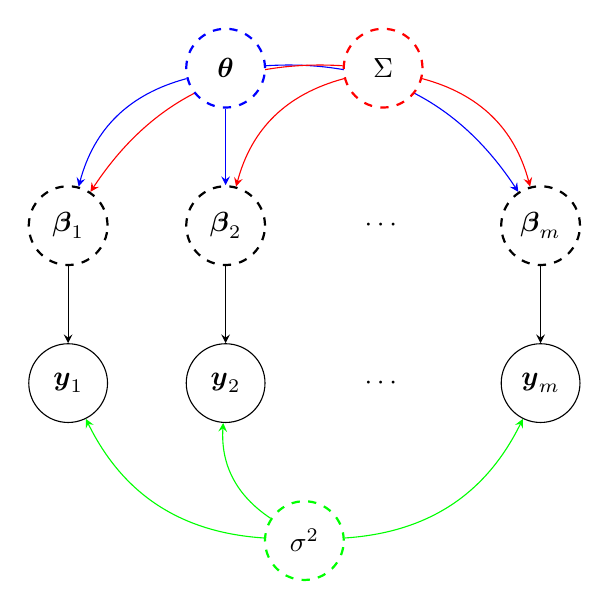
\begin{tikzpicture}[node distance=2cm,->,>=stealth]
 % styles
 \tikzstyle{param} = [circle,thick,draw=black,fill=white,dashed,minimum size=1cm];
 \tikzstyle{yobs} = [circle,draw=black,fill=white,minimum size=1cm];

 % nodes
 \node[param,draw=blue] (theta) {$ \vect \theta $};
 \node[param,right of=theta,draw=red] (Sigma) {$ \Sigma $};
 \node[param,below of=theta] (beta2) {$ \vect \beta_2 $};
 \node[param,left of=beta2]  (beta1) {$ \vect \beta_1 $};
 \node[param,below of=Sigma,draw=white] (betadot) {$ \cdots $};
 \node[param,right of=betadot] (betam) {$ \vect \beta_m $};
 \node[yobs,below of=beta1] (y1) {$ \vect y_1 $};
 \node[yobs,below of=beta2] (y2) {$ \vect y_2 $};
 \node[yobs,below of=betadot,draw=white] (ydot) {$ \cdots $};
 \node[yobs,below of=betam] (ym) {$ \vect y_m $};
 
 \node[param,below of=y2,xshift=1cm,draw=green] (sigma2) {$ \sigma ^2 $};

 \begin{pgfonlayer}{background}
 % edges
 \path [blue] (theta)
       edge [bend right] node {} (beta1)
       edge node {} (beta2)
       edge [bend left]  node {} (betam);

 \path [red] (Sigma)
       edge [bend right] node {} (beta1)
       edge [bend right] node {} (beta2)
       edge [bend left]  node {} (betam);

 \path [green] (sigma2)
       edge [bend left]  node {} (y1)
       edge [bend left]  node {} (y2)
       edge [bend right] node {} (ym);

 \path (beta1) edge node {} (y1);
 \path (beta2) edge node {} (y2);
 \path (betam) edge node {} (ym);
 \end{pgfonlayer}
 \end{tikzpicture}
\end{figure}
\begin{align*}
 \vect \theta & \sim \Normal_{p}(\mu_0, \Lambda_0) \\
 \Sigma & \sim \invWishart(\eta_0, S_0 ^{-1}) \\
 \sigma ^2 & \sim \invGamma(\nu_0 / 2, \nu_0 \sigma_0 ^2 / 2) \\
 \vect \beta_j | \vect \theta, \Sigma & \sim \Normal_{p}(\vect \theta, \Sigma) \\
 \vect y_j | \beta_j, \sigma^2 & \sim \Normal_{n_j}(X_j \vect \beta_j, \sigma ^2 \cdot \Imat)
\end{align*}
\[ p(\vect \theta, \Sigma, \sigma ^2, \vect \beta_1, \ldots, \vect \beta_m, \vect y_1, \ldots, \vect y_m) = 
   p(\vect \theta) \cdot p(\vect \Sigma) \cdot p(\sigma ^2) \cdot 
   \prod_j p(\vect \beta_j | \vect \theta, \Sigma) \cdot 
   \prod_j p(\vect y_j | \beta_j, \sigma ^2) \]
Now we can derive the full conditional distributions of the stochastic system
parameters as required:

\subsubsection{Full conditional of $ \vect \beta_j $}
\begin{align*}
 p(\vect \beta_j | \vect \beta_{-j}, \vect \theta, \Sigma, \sigma ^2, \vect y_1, \ldots, \vect y_m)
  &= p(\vect \beta_j | \vect \theta, \Sigma, \sigma ^2, \vect y_j) \\
  &\propto p(\vect \beta_j | \vect \theta, \Sigma) \cdot p(\vect y_j | \vect \beta_j, \sigma ^2) \\
  &\propto \frac{1}{\sqrt{(2 \pi) ^{p} \left|\Sigma\right|}} \cdot 
          \exp\left( -\frac{1}{2} (\vect \beta_j - \vect \theta)' \Sigma ^{-1} (\vect \beta_j - \vect \theta) \right) \cdot \\
  &\phantom= \frac{1}{\sqrt{(2 \pi \sigma ^2) ^{n_j}}} \cdot 
           \exp\left( -\frac{1}{2 \sigma ^2} (\vect y_j - X_j \vect \beta_j)' (\vect y_j - X_j \vect \beta_j) \right) \\
  &\propto \exp\left\{ -\frac{1}{2} 
               \left(\vect \beta_j' \Sigma ^{-1} \vect \beta_j - 2 \vect \beta_j' \Sigma ^{-1} \vect \theta +
                     \vect \theta' \Sigma ^{-1} \vect \theta + \frac{\vect y_j' \vect y_j}{\sigma ^2} - 
                     2 \vect \beta_j' \frac{X_j' \vect y_j}{\sigma ^2} + \vect \beta_j' \frac{X_j' X_j}{\sigma ^2} \vect \beta_j
               \right) \right\} \\
  &\propto \exp\left\{ -\frac{1}{2} \left[ 
                      \vect \beta_j' \left(\Sigma ^{-1} + \frac{X_j' X_j}{\sigma ^2}\right) \vect \beta_j -
                      2 \vect \beta_j' \left( \Sigma ^{-1} \vect \theta + \frac{X_j' \vect y_j}{\sigma ^2} \right)
                                    \right] \right\}
\end{align*}
We can extrapolate the kernel of a multivariate normal distribution, thus:
\[ \vect \beta_j | \vect \theta, \Sigma, \sigma ^2, \vect y_j \sim 
   \Normal_p\left( \left( \Sigma ^{-1} + \frac{X_j' X_j}{\sigma ^2} \right) ^{-1}
                   \left( \Sigma ^{-1} \vect \theta + \frac{X_j' \vect y_j}{\sigma ^2} \right), 
                   \left( \Sigma ^{-1} + \frac{X_j' X_j}{\sigma ^2} \right) ^{-1} \right) \]

\subsubsection{Full conditional of $ \vect \theta $}
\begin{align*}
 p(\vect \theta | \vect \beta_1, \ldots, \vect \beta_m, \Sigma, \sigma ^2, \vect y_1, \ldots, \vect y_m)
  &= p(\vect \theta | \vect \beta_1, \ldots, \vect \beta_j, \Sigma) \\
  &\propto p(\vect \theta) \cdot \prod_j p(\vect \beta_j | \vect \theta, \Sigma) \\
  &\propto \frac{1}{\sqrt{(2 \pi) ^p \left| \Lambda_0 \right|}} \cdot
           \exp\left( -\frac{1}{2} (\vect \theta - \vect \mu_0)' \Lambda_0 ^{-1} (\vect \theta - \vect \mu_0) \right) \cdot \\
  & \prod_j \frac{1}{\sqrt{(2 \pi) ^p \left| \Sigma \right|}} \cdot
            \exp\left( -\frac{1}{2} (\vect \beta_j - \vect \theta)' \Sigma ^{-1} (\vect \beta_j - \vect \theta) \right) \\
  &\propto \exp\left\{ -\frac{1}{2} \left(
                      \vect \theta' \Lambda_0 ^{-1} \vect \theta - 2 \vect \theta' \Lambda_0 ^{-1} \vect \mu_0 + 
                      \vect \mu_0' \Lambda_0 ^{-1} \vect \mu_0 \right) \right\} \cdot \\
  &\phantom\prod \exp\left\{ -\frac{m}{2} \left(
                        \vect \theta' \Sigma ^{-1} \vect \theta - 2 \vect \theta' \Sigma ^{-1} \vect{\bar \beta} +
                        \vect{\bar \beta} \Sigma ^{-1} \vect{\bar \beta}
                 \right) \right\} \\
  &\propto \exp\left\{ -\frac{1}{2} \left[
                      \vect \theta' \left( \Lambda_0 ^{-1} + m \Sigma ^{-1} \right) \vect \theta -
                      2 \vect \theta' \left( \Lambda_0 ^{-1} \vect \mu_0 + m \Sigma ^{-1} \vect{\bar \beta} \right)
               \right] \right\}
\end{align*}
We can note the kernel of a multivariate normal distribution:
\[ \vect \theta | \vect \beta_1, \ldots, \vect \beta_j, \Sigma \sim
   \Normal_p\left( \left( \Lambda_0 ^{-1} + m \Sigma ^{-1} \right) ^{-1}
                   \left( \Lambda_0 ^{-1} \vect \mu_0 + m \Sigma ^{-1} \vect{\bar \beta} \right),
                   \left( \Lambda_0 ^{-1} + m \Sigma ^{-1} \right) ^{-1} \right) \]

\subsubsection{Full conditional of $ \Sigma $}
\setlength{\fboxsep}{10pt} % increase the spacing of fbox
\begin{align*}
 p(\Sigma | \vect \theta, \sigma ^2, \vect \beta_1, \ldots, \vect \beta_m, \vect y_1, \ldots, \vect y_m) 
  &= p(\Sigma | \vect \beta_1, \ldots, \vect \beta_m, \vect \theta) \\
  &\propto p(\Sigma) \cdot \prod_j p(\vect \beta_j | \vect \theta, \Sigma) \\
  &\propto \left( 2 ^{\frac{\eta_0 p}{2}} \pi ^{\binom{p}{2} / 2} \cdot \left| S_0 \right| ^{-\frac{\eta_0}{2}} 
           \prod_{k = 1}^{p} \frac{\eta_0 + 1 - k}{2} \right) ^{-1} \cdot
           \left| \Sigma \right| ^{-\frac{\eta_0 + p + 1}{2}} e ^{\frac{1}{2} \tr(S_0 \Sigma ^{-1})} \cdot \\
  & \prod_j \frac{1}{\sqrt{(2 \pi) ^p \left| \Sigma \right|}} \cdot 
            \exp\left( -\frac{1}{2} (\vect \beta_j - \vect \theta)' \Sigma ^{-1} (\vect \beta_j - \vect \theta) \right) \\
  &\propto \left| \Sigma \right| ^{-\frac{\eta_0 + p + 1}{2}} \exp \left( -\frac{1}{2} \tr\left( S_0 \Sigma ^{-1} \right) \right)
           \left| \Sigma \right| ^{-\frac{m}{2}} \exp\left( -\frac{1}{2} \sum_j (\vect \beta_j - \vect \theta)' \Sigma ^{-1} 
           (\vect \beta_j - \vect \theta) \right) \\
  \intertext{\centering \fbox{\parbox{0.5\textwidth}{
             Considering that \begin{align*}
                \sum_j (\vect \beta_j - \vect \theta)' \Sigma ^{-1} (\vect \beta_j - \vect \theta) 
                  &= \sum_j \tr((\vect \beta_j - \vect \theta)' \Sigma ^{-1} (\vect \beta_j - \vect \theta)) \\
                  &= \sum_j \tr((\vect \beta_j - \vect \theta) (\vect \beta_j - \vect \theta)' \Sigma ^{-1}) \\
                  &= \tr\left( \sum_j (\vect \beta_j - \vect \theta) (\vect \beta_j - \vect \theta)' \Sigma ^{-1} \right) \\
                  &= \tr(S_{\beta} \Sigma ^{-1})
             \end{align*}}}} \\
  &= \left| \Sigma \right| ^{-\frac{\eta_0 + p + m + 1}{2}} \cdot 
     \exp\left( -\frac{1}{2} \tr\left((S_0 + S_\beta) \Sigma ^{-1}\right) \right)
\end{align*}
We recognize the kernel of an inverse-Wishart:
\[ \Sigma | \vect \beta_1, \ldots, \vect \beta_m, \vect \theta \sim 
   \invWishart\left( \eta_0 + m, (S_0 + S_\beta) ^{-1} \right) \]

\subsubsection{Full conditional of $ \sigma ^2 $}
\begin{align*}
 p(\sigma ^2 | \vect \theta, \Sigma, \vect \beta_1, \ldots, \vect \beta_m, \vect y_1, \ldots, \vect y_m)
  &= p(\sigma ^2 | \vect \beta_1, \ldots, \vect \beta_j, \vect y_1, \ldots, \vect y_m) \\
  &\propto p(\sigma ^2) \cdot \prod_j p(\vect y_j | \sigma ^2, \vect \beta_j) \\
  &= \frac{\left( \frac{\nu_0 \sigma_0 ^2}{2} \right) ^{\frac{\nu_0}{2}}}{\Gamma\left( \frac{\nu_0}{2} \right)} \cdot
     (\sigma ^2) ^{- \left(\frac{\nu_0}{2} + 1\right)} \exp\left( -\frac{\nu_0 \sigma_0 ^2}{2 \sigma ^2} \right) \cdot \\
  & \prod_j \frac{1}{\sqrt{(2 \pi \sigma ^2) ^{n_j}}} \cdot 
    \exp\left( -\frac{1}{2 \sigma ^2} (\vect y_j - X_j \vect \beta_j)' (\vect y_j - X_j \vect \beta_j) \right) \\
  &\propto (\sigma ^2) ^{- \left[ \frac{1}{2} \left( \nu_0 + \sum_j n_j \right) + 1 \right]} \cdot
           \exp\left\{ -\frac{1}{2 \sigma ^2} \left[ \nu_0 \sigma_0 ^2 + 
           \textstyle \sum_j (\vect y_j - X_j \vect \beta_j)' (\vect y_j - X_j \vect \beta_j) \right]\right\}
\end{align*}
We recognize the kernel of an inverse-Gamma distribution:
\[ \sigma ^2 | \vect \beta_1, \ldots, \vect \beta_m, \vect y_1, \ldots, \vect y_m \sim
   \invGamma\left( \frac{1}{2} \left( \nu_0 + \textstyle \sum_j n_j \right),
                   \frac{1}{2} \left( \nu_0 \sigma_0 ^2 + 
                   \textstyle \sum_j (\vect y_j - X_j \vect \beta_j)' (\vect y_j - X_j \vect \beta_j) \right) \right) \]

\section{Exercise 11.4, Hoff}

\subsection{Data}
Hierarchical logistic regression: The Washington Assessment of Student Learning
(WASL) is a standardized test given to students in the state of Washington.
Letting j index the counties within the state of Washington and i index schools
within counties, the file \texttt{mathstandard.dat} includes data on the
following variables:
\begin{itemize}
 \item $ y_{i, j} = $ the indicator that more than half the 10th graders in
 school i, j passed the WASL math exam;
 \item $ x_{i, j} = $ the percentage of teachers in school i, j who have a
 masters degree.
\end{itemize}
In this exercise we will construct an algorithm to approximate the posterior
distribution of the parameters in a generalized linear mixed-effects model for
these data. The model is a mixed effects version of logistic regression:
\begin{align*}
 y_{i, j} &\sim \Binomial(e ^{\eta_{i, j} / (1 + \eta_{i, j})}) 
  &\text{ where }& \quad \eta_{i, j} = \beta_{0, j} + \beta_{1, j} x_{i, j} \\
 \vect \beta_1, \ldots, \vect \beta_m &\sim \Normal_{p}(\vect \theta, \Sigma)
  &\text{ where }& \quad \vect \beta_j = \begin{pmatrix} \beta_{0, j} \\ \beta_{1, j} \end{pmatrix}
\end{align*}

\subsection{Questions}
\begin{enumerate}[label=\alph*) ]
 \item The unknown parameters in the model include population-level parameters $
 \{\vect \theta, \Sigma\} $ and the group level parameters $ \{\vect \beta_1,
 \ldots, \vect \beta_m\} $. Draw a diagram that describes the relationships
 between these parameters, the data $ \{ y_{i, j}, x_{i, j} \} $ and prior
 distributions.
 \item Before we do a Bayesian analysis, we will get some ad hoc estimates of
 these parameters via maximum likelihood: fit a separate logistic regression
 model for each group, possibly using the \texttt{glm} command in R via
 \texttt{beta.j <- glm(y.j $\sim$ X.j, family = binomial())\$coef}. Explain any
 problems you have with obtaining estimates for each county. Plot $ \expit(-\hat
 \beta_{0, j} - \hat \beta_{1, j} x) $ as a function of $ x $ for each county
 and describe what you see. Using maximum likelihood estimates only from those
 counties with 10 or more schools, obtain ad hoc estimates $ \hat{\vect \theta}
 $ and $ \hat{\Sigma} $ of $ \vect \theta $ and $ \Sigma $. Note that these
 estimates may not be representative of patterns from schools with small sample
 sizes.
 \item Formulate a unit information prior distribution for $ \vect \theta $ and
 $ \Sigma $ based on the observed data. Specifically, let $ \vect \theta \sim
 \Normal_p(\hat{\vect{\theta}}, \Sigma) $ and let $ \Sigma ^{-1} \sim
 \invWishart(4, \hat{\Sigma} ^{-1}) $. Use a Metropolis-Hastings algorithm to
 approximate the joint posterior distribution of all parameters.
 \item Make plots of the samples of $ \vect \theta $ and $ \Sigma $ (5
 parameters) versus MCMC iteration number. Make sure you run the chain long
 enough so that your MCMC samples are likely to be a reasonable approximation to
 the posterior distribution.
 \item Obtain posterior expectations of $ \vect \beta_j $ for each group $ j $,
 plot $ \E[\beta_{0, j} | \vect y] + \E[\beta_{1, j} | \vect y] x $ as a
 function of $ x $ for each county, compare to the plot in b) and describe why
 you see any differences between the two sets of regression lines.
 \item From your posterior samples, plot marginal posterior and prior densities
 of $ \vect \theta $ and the elements of $ \Sigma $. Include your ad hoc
 estimates from b) in the plots. Discuss the evidence that the slopes or
 intercepts vary across groups.
\end{enumerate}

\subsection{Solutions}
\begin{enumerate}[label=\alph*) ]
 \item The DAG of the model has the common hierarchical shape:
 \begin{figure}[H]
  \centering
  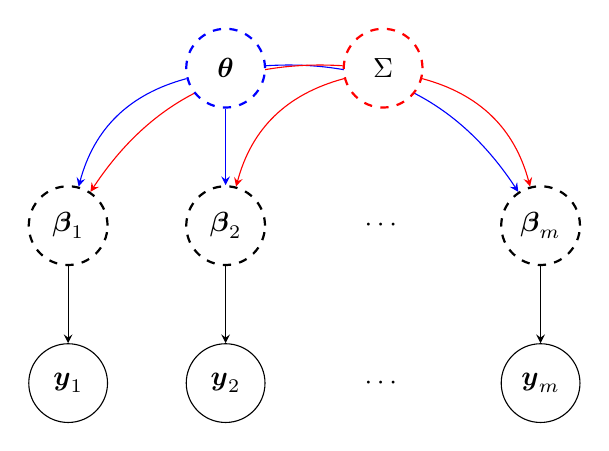
\begin{tikzpicture}[node distance=2cm,->,>=stealth]
  % styles
  \tikzstyle{param} = [circle,thick,draw=black,fill=white,dashed,minimum size=1cm];
  \tikzstyle{yobs} = [circle,draw=black,fill=white,minimum size=1cm];
 
  % nodes
  \node[param,draw=blue] (theta) {$ \vect \theta $};
  \node[param,right of=theta,draw=red] (Sigma) {$ \Sigma $};
  \node[param,below of=theta] (beta2) {$ \vect \beta_2 $};
  \node[param,left of=beta2]  (beta1) {$ \vect \beta_1 $};
  \node[param,below of=Sigma,draw=white] (betadot) {$ \cdots $};
  \node[param,right of=betadot] (betam) {$ \vect \beta_m $};
  \node[yobs,below of=beta1] (y1) {$ \vect y_1 $};
  \node[yobs,below of=beta2] (y2) {$ \vect y_2 $};
  \node[yobs,below of=betadot,draw=white] (ydot) {$ \cdots $};
  \node[yobs,below of=betam] (ym) {$ \vect y_m $};
 
  \begin{pgfonlayer}{background}
  % edges
  \path [blue] (theta)
        edge [bend right] node {} (beta1)
        edge node {} (beta2)
        edge [bend left]  node {} (betam);
 
  \path [red] (Sigma)
        edge [bend right] node {} (beta1)
        edge [bend right] node {} (beta2)
        edge [bend left]  node {} (betam);
 
  \path (beta1) edge node {} (y1);
  \path (beta2) edge node {} (y2);
  \path (betam) edge node {} (ym);
  \end{pgfonlayer}
  \end{tikzpicture}
 \end{figure}
  \begin{align*}
    \vect \theta & \sim \Normal_p (\mu_0, \Lambda_0) \\
    \Sigma & \sim \invWishart (\eta_0, S_0 ^{-1}) \\
    \vect \beta_j | \vect \theta, \Sigma & \sim \Normal_p (\vect \theta, \Sigma) \\
    \vect y_j | \vect \beta_j & \sim \Bernoulli_{n_j} (\expit (X_j \vect \beta_j))
  \end{align*}
  \item Code (results in figure \ref{week10:groupedglm}):
\begin{minted}{R}

library(tidyverse)
library(mvnfast)
library(compiler)

invlogit <- function(x) 1 / (1 + exp(-x))

# Load data
mathstandard <- read.table("data/mathstandard2.dat", header = TRUE)

# b)
GLMfits <- by(mathstandard, with(mathstandard, county), function(data)
   glm(metstandard ~ percentms, family = binomial(), data = data))

Beta     <- t(sapply(GLMfits, coefficients))
n        <- with(mathstandard, table(county))
topn     <- n %>% keep(~ . >= 10)
ML_theta <- Beta[names(topn), ] %>% colMeans
ML_Sigma <- Beta[names(topn), ] %>% cov

palette(grey.colors(max(n), 0.8, 0))

pdf("week-10_groupedglm.pdf", height = 5)

plot(c(0, 100), c(0, 1), type = 'n', bty = 'n',
     xlab = "teachers with MS (%)", ylab = "P(Y = 1)")
for (i in 1:NROW(Beta)) {
   curve(invlogit(Beta[i, 1] + Beta[i, 2] * x), add = TRUE, col = n[i])
}

curve(invlogit(ML_theta[1] + ML_theta[2] * x), add = TRUE,
      col = "red", lty = 2, lwd = 4)

graphics.off()

pdf("week-10_frequencies.pdf", height = 4)
tibble(county = names(n), freq = n, min5 = factor(n < 5)) %>%
   ggplot(aes(county, freq, fill = min5)) +
   geom_col(show.legend = FALSE) +
   theme_minimal() + scale_fill_manual(values = c("#1E90FF", "#FF0000")) +
   theme(axis.text.x = element_text(angle = 90)) +
   ylab("Frequency") + xlab("County")
graphics.off()
\end{minted}

  \begin{figure}
    \centering
    \includegraphics[width=0.8\linewidth]{r-scripts/week-10_groupedglm.pdf}
    \caption{Maximum likelihood estimation model by group in scales of gray (the
    darker the line the more numerous group). Average coefficients for groups
    larger than 10 elements in red dashed line.}
    \label{week10:groupedglm}
  \end{figure}
  Using classical GLM estimation \textit{by group} gives rise to a number of
  problems: first of all, we can see that many groups have a very low number of
  observations, as we can see in figure \ref{week10:frequencies}, and thus the
  maximum likelihood estimates have a high variance and a high numerical
  instability. For the low number of observations, there is another possible
  obstacle: if the observations are perfectly separable the Fisher scoring
  algorithm does not converge and we have a missing value in place of the
  coefficient. In figure \ref{week10:groupedglm} we can observe that many curves
  have a very irregular trend, some are in total contradiction with the others
  (some show a direct relation, other an inverse), and it is very difficult to
  understand which is the \textit{neat} relation. The maximum likelihood
  estimation leads to the red dashed line, which seems to be influenced mostly
  from the more regular curves, in fact, to calculate it we have considered only
  larger groups.
  \begin{figure}
    \centering
    \includegraphics[width=0.8\linewidth]{r-scripts/week-10_frequencies.pdf}
    \caption{Frequencies of observations within counties. Red bars have an
    absolute frequency below 5, blue bars above.}
    \label{week10:frequencies}
  \end{figure}

 \item Code:
\begin{minted}{R}
Y <- with(mathstandard, tapply(metstandard, county, identity))
X <- with(mathstandard, split(mathstandard, county)) %>%
   map(~ model.matrix(metstandard ~ percentms, data = .))

p <- 2
m <- length(X)

simulateMH <- function(niter, init, seed = NULL) {
   set.seed(seed)

   # Hyperparameters
   mu0   <- init$mu
   S0    <- init$S
   eta0  <- init$eta
   Beta  <- init$Beta
   invL0 <- invSigma <- solve(S0)

   # Init storing variables
   THETA <- matrix(NA, niter, p)
   BETA  <- array(NA, c(m, p, niter))
   SIGMA <- array(NA, c(p, p, niter))

   colnames(THETA) <- names(mu0)
   dimnames(BETA)  <- dimnames(Beta)
   dimnames(SIGMA) <- dimnames(S0)

   for (itr in 1:niter) {
      # update theta
      Lm    <- solve(invL0 + m * invSigma)
      mu_m  <- Lm %*% (invL0 %*% mu0 + invSigma %*% colSums(Beta))
      theta <- rmvn(1, mu_m, Lm) %>% drop()

      # update Sigma
      tmp      <- sweep(Beta, 2, theta)
      invSigma <- rWishart(1, eta0 + m, solve(S0 + crossprod(tmp))) %>% drop()
      Sigma    <- solve(invSigma)

      # update Beta
      Beta0      <- tapply(Beta, row(Beta), t)
      Beta1      <- tapply(Beta, row(Beta), rmvn, n = 1, sigma = Sigma / 2)
      lpBeta0    <- sapply(Beta0, dmvn, theta, Sigma, log = TRUE)
      lpBeta1    <- sapply(Beta1, dmvn, theta, Sigma, log = TRUE)
      pi.Beta0   <- mapply(tcrossprod, X, Beta0, SIMPLIFY = FALSE) %>% lapply(invlogit)
      pi.Beta1   <- mapply(tcrossprod, X, Beta1, SIMPLIFY = FALSE) %>% lapply(invlogit)
      lpyi.Beta0 <- mapply(dbinom, Y, pi.Beta0, MoreArgs = list(size = 1, log = TRUE), 
                           SIMPLIFY = FALSE)
      lpyi.Beta1 <- mapply(dbinom, Y, pi.Beta1, MoreArgs = list(size = 1, log = TRUE),
                           SIMPLIFY = FALSE)

      lr <- sapply(lpyi.Beta1, sum) - sapply(lpyi.Beta0, sum) + lpBeta1 - lpBeta0
      lu <- log(runif(m))
      Beta[lu < lr, ] <- do.call(rbind, Beta1[lu < lr])

      THETA[itr, ]   <- theta
      BETA[, , itr]  <- Beta
      SIGMA[, , itr] <- Sigma
   }

   # [return]
   list(THETA = THETA, SIGMA = SIGMA, BETA = BETA)
}

init  <- list(mu = ML_theta, S = ML_Sigma, eta = 4, Beta = replace_na(Beta, 0))
niter <- 10000

mcmcsim <- simulateMH(niter, init)
\end{minted}

 \item Code (results in figure \ref{week10:mcmcplots}):
\begin{minted}{R}
B <- 500 # burn-in

pdf("week-10_mcmcplot.pdf", height = 9)

mcmcsim %$%
   tibble(`theta[intercept]`   = THETA[, 1],
          `theta[percentms]`   = THETA[, 2],
          `sigma[intercept]^2` = SIGMA[1, 1, ],
          `sigma[int * pms]`   = SIGMA[1, 2, ],
          `sigma[percentms]^2` = SIGMA[2, 2, ],
          iteration            = seq_len(niter),
          status               = factor(iteration < B, c(TRUE, FALSE),
                                        c("`Burn-in`", "Warmed"))) %>%
   gather(param, value, -iteration, -status) %>%
   ggplot(aes(iteration, value)) + geom_line() +
   facet_wrap(~ param + status, nc = 2, scale = "free",
              labeller = label_parsed) +
   theme_minimal() + ylab("") + xlab("")

graphics.off()
\end{minted}
 \begin{figure}
  \centering
  \includegraphics[width=\linewidth]{r-scripts/week-10_mcmcplot.pdf}
  \caption{Chains for the 5 parameters, divided in burn-in period and warmed period.}
  \label{week10:mcmcplots}
 \end{figure}

 \item Code (results in \ref{week10:groupedposterior}):
\begin{minted}{R}
E_Beta  <- mcmcsim %$% apply(BETA[, , B:niter], 1:2, mean)
E_Sigma <- mcmcsim %$% apply(SIGMA[, , B:niter], 1:2, mean)
E_theta <- mcmcsim %$% colMeans(THETA[B:niter, ])
V_theta <- mcmcsim %$% cov(THETA[B:niter, ])

pdf("week-10_groupedposterior.pdf", height = 5)

plot(c(0, 100), c(0, 1), type = 'n', bty = 'n',
     xlab = "teachers with MS (%)", ylab = "P(Y = 1)")
for (i in 1:NROW(E_Beta)) {
   curve(invlogit(E_Beta[i, 1] + E_Beta[i, 2] * x), add = TRUE, col = n[i])
}

curve(1 / (1 + exp(-E_theta[1] - E_theta[2] * x)), add = TRUE,
      col = "red", lty = 2, lwd = 3)
curve(1 / (1 + exp(-ML_theta[1] - ML_theta[2] * x)), add = TRUE,
      col = "brown", lty = 3, lwd = 3)

graphics.off()
\end{minted}

 \begin{figure} 
  \centering
  \includegraphics[width=0.8\linewidth]{r-scripts/week-10_groupedposterior.pdf}
  \caption{Expected parameters given the $ \vect y_j $ by group in scales of
  gray (the darker the line the more numerous the group). Expected value for $
  \vect \theta $ in dashed red and MLE of $ \vect \theta $ (same as
  \ref{week10:groupedglm}) in dotted brown.}
  \label{week10:groupedposterior}
 \end{figure}

 \item Code (results in figure \ref{week10:priorvsposterior}):
 \begin{figure}[H]
  \centering
  \includegraphics[width=\linewidth]{r-scripts/week-10_prior_posterior-1.pdf}
  \label{week10:priorvsposterior}
 \end{figure}
\end{enumerate}
\end{document}
